\documentclass[12pt, letterpaper, onecolumn, conference, final]{IEEEtran}

\usepackage[margin = .5in]{geometry}
\usepackage{amsmath}
\usepackage{amsthm}
\usepackage{amssymb}
\usepackage{wasysym}
\usepackage[utf8]{inputenc}
\usepackage[linktocpage=true]{hyperref}
\usepackage{graphicx}
\usepackage{fancyhdr}

\theoremstyle{definition}
\newtheorem{definition}{Definition}[section]
\newtheorem{lemma}{Lemma}[section]

\theoremstyle{plain}
\newtheorem{example}{Example}[section]
\newtheorem{solution}{Solution}[section]

\renewcommand\thesection{\arabic{section}}

\renewcommand\qedsymbol{$\blacksquare$}

\title{Combinatorics \& Graph Theory Notes}
\author{Based on Lectures Given by James Frauenthal \\ Spring 2013}

\usepackage[T1]{fontenc}

\usepackage[tocflat]{tocstyle}
\usetocstyle{standard}

\usepackage{blindtext}

% Redefinition of ToC command to get centered heading
\makeatletter
\renewcommand\tableofcontents{%
  \null\hfill\textbf{\Large\contentsname}\hfill\null\par
  \@mkboth{\MakeUppercase\contentsname}{\MakeUppercase\contentsname}%
  \@starttoc{toc}%
}

\pagestyle{fancy}
\fancyhf{}
\lhead{Page \thepage}

\begin{document}

\maketitle

\tableofcontents

\newpage

\setcounter{page}{1}

\section{\textbf{\underline{Combinatorics - Introduction}}}
\vspace{.3cm}
\noindent
We will start out learning how to count. To dispel the notion that this is trivial consider the following problems.

\begin{example}[The Tennis Tournament]
A tennis tournament works as follows. All the names of contestants are placed in a hat and withdrawn in pairs. Each pair plays a set and the winners' names are returned to the hat. If an odd number of names are in the hat, the last remaining name is given a "bye" (and thus simply left in the hat until the next round). How many matches (sets) will be played if $N$ people enter?
\end{example}
\begin{solution}[The Tennis Tournament]
Consider by examples:
\begin{eqnarray}
N=32 \implies 16+8+4+2+1&=31 \nonumber \\
N=57 \implies 28+14+7+4+2+1&=56 \nonumber
\end{eqnarray}
Now stop and think of a cleaner way. If $N$ people enter the tournament and only one person (the winner) never loses a match this implies all others lose exactly one match and thus there must be $N-1$ matches.
\end{solution}

\begin{example}[The Peg Game]
Given a board with 9 holes in a row with 4 black pegs at one end and 4 blue pegs at the other end. The object of the game is to switch the pegs so that the blue pegs occupy the holes where the black pegs start and vise versa. The following rules must be followed:
\begin{center}
\begin{tabular}{| l | l |}
\hline
Rule 1: & Only one peg moves at a time \\ \hline
Rule 2: & Pegs may only advance, never retreat \\ \hline
Rule 3: & Pegs move only one space at a time (unless they jump) \\ \hline
Rule 4: & Pegs may only jump pegs of the other color and may only jump one peg at a time \\ \hline
\end{tabular}
\end{center}
Ordinarily one tries to figure out how to play the game. We assume a unique solution is possible and try to figure out how many moves it takes to finish the game.
\end{example}

\vspace{.3cm}
\section{\textbf{\underline{Why Do We Want to Know How to Count?}}}
\vspace{.3cm}
\noindent
Perhaps the best simple answer is that it is often necessary if we wish to determine probabilities. Imagine that we do an "experiment" such as tossing a die. We distinguish in this case the 6 elementary events (i.e. get a 1,2,3,4,5, or 6).

\begin{center}
\fbox{
\begin{minipage}{7.3 in}
\begin{definition}[Laplace's Interpretation of Probability]
If:
\begin{center}
\begin{tabular}{l l}
1: & There are a finite number of elementary events - say $n$ \\
2: & The elementary events are equally likely \\
3: & The event of interest $A$ can be uniquely decomposed into $m$ elementary events where $m \leq n$ \\
\end{tabular}
\end{center}
then:
\begin{eqnarray}
\mathbb{P}[A] = \frac{m}{n} \nonumber 
\end{eqnarray}
where:
\begin{center}
\begin{tabular}{l l}
1: & $0 \leq \mathbb{P}[A] \leq 1$ \\
2: & $\mathbb{P}[A] = 1$ iff $m=n$ \\
3: & $\mathbb{P}[A] = 0$ iff $m=0$ \\
\end{tabular}
\end{center}
\end{definition}
\end{minipage}}
\end{center}

\noindent
Although apparently simple, Laplace's definition is not without pitfalls. The most serious concerns arise with condition 2. How do we decide if events are equally likely? This is a topic for a statistics course and thus we will hypothesize that fairs coins, dice, \dots exist, at least in theory even if we do not know how to prove their existence. In the following examples let $H = \#$ of heads and $T = \#$ of tails.

\begin{example}
A fair coin is tossed once. What is $\mathbb{P}[H = 1]$?
\end{example}

\newpage
\begin{solution}
Clearly Laplace's definition is satisfied and in this case $n=2$ since there are a total of 2 elementary events and our event of choice is one of them implying that $m=1$. Thus $\mathbb{P}[H = 1] = \frac{m}{n} = \frac{1}{2}$.
\end{solution}

\begin{example}
A fair coin is tossed twice. What is $\mathbb{P}[H \geq 1]$?
\end{example}
\begin{solution}
Clearly Laplace's definition is satisfied and in this case $n=4$ since there are a total of 4 possible outcomes: $(H,H), (H,T), (T,H), (T,T)$. Of these $m=3$ have at least one head. Therefore, $\mathbb{P}[H \geq 1] = \frac{m}{n} = \frac{3}{4}$.
\end{solution}

\noindent
Note that $(H,H), (H,T), (T,H), (T,T)$ are the elementary events here. Other questions we might have asked are $\mathbb{P}[H = 1] = \frac{2}{4} = \frac{1}{2}$ or $\mathbb{P}[H = 0] = \mathbb{P}[T = 2] = \frac{1}{4}$. Can we use this example to illustrate where Laplace's predecessors went wrong. Jean le Rond d'Alembert (1717 - 1783) said: "Could toss a head and thus not need to toss again, or toss a tail followed by a head or a tail followed by a tail" $\implies \mathbb{P}[H \geq 1] = \frac{2}{3}$. His view was wrong because he did not consider all of the events.

\begin{example}
A fair die is tossed. Let $O$ represent the event of getting an odd number. What is $\mathbb{P}[O]$?
\end{example}
\begin{solution}
Decompose the compound event $O$ into the elementary events 1,3, or 5. Thus $m=3$, $n=6$, and $\mathbb{P}[O] = \frac{m}{n} = \frac{3}{6} = \frac{1}{2}$.
\end{solution}

\vspace{.3cm}
\section{\textbf{\underline{Two Counting Principles}}}
\vspace{.3cm}
\begin{center}
\fbox{
\begin{minipage}{7.3 in}
\begin{definition}[Counting Principles]
Imagine that we have available 4 kinds of breakfast cereal $A$ and 3 kinds of fruit $B$. How many ways can we select a cereal \underline{and} a fruit $(A \cap B)$? How many ways can we select a cereal \underline{or} a fruit $(A \cup B)$? More generally, imagine event $A$ occurs $a$ different ways, event $B$ occurs $b$ different ways, \dots, and event $H$ occurs $h$ different ways, then:
\begin{eqnarray}
A \cap B \cap \dots \cap H \text{ occurs } a \times b \times \dots \times h \text{ ways} \nonumber \\
A \cup B \cup \dots \cup H \text{ occurs } a+b+\dots +h \text{ ways} \nonumber
\end{eqnarray}
\end{definition}
\end{minipage}}
\end{center}

\begin{example}
Two dice are tossed (1 Red, 1 Green). How many ways can they fall?
\end{example}
\begin{solution}
Let the event $A$ represent how many ways the red die can fall and $B$ represent the number of ways the green die can fall. Each can fall 6 ways, therefore, $A \cap B = 6 \cdot 6 = 36$. 
\end{solution}

\begin{example}
Now lets consider a more general case where we have 10 distinguishable dice. How many ways can they fall?
\end{example}
\begin{solution}
Let the event $A_1$ represent how many ways the first die can fall, $A_2$ represent the number of ways the second die can fall, \dots, and $A_{10}$ represent how many ways the tenth die can fall. Each can fall 6 ways, therefore, $A_1 \cap A_2 \cap \dots \cap A_{10} = 6^{10} = 60,466,176$ ways. 
\end{solution}

\begin{example}
Six letters are placed into six envelopes such that each envelope contains one letter. How many ways can this be done?
\end{example}
\begin{solution}
Let the event $A_1$ represent the number of ways of picking one letter of the six letters for the first envelope, $A_2$ represent the number of ways of picking one of the five remaining letters for the second envelope, \dots, and $A_6$ represent the number of ways of picking one of the one remaining letters for the sixth envelope. Therefore, $A_1 \cap A_2 \cap \dots \cap A_{6} = 6 \cdot 5 \cdot 4 \cdot 3 \cdot 2 \cdot 1 = 6! = 720$ ways.
\end{solution}

\begin{example}
Out of the four digits 1,2,3, and 4, how many numbers can we construct which have no repeated digits?
\end{example}

\newpage
\begin{solution}
Lets model all the different cases in a table:
\begin{center}
\begin{tabular}{| c | l |}
\hline
Length of Number & \# of Orderings \\ \hline
1 & 4 \\ \hline
2 & 4 $\cdot$ 3 = 12 \\ \hline
3 & 4 $\cdot$ 3 $\cdot$ 2 = 24 \\ \hline
4 & 4 $\cdot$ 3 $\cdot$ 2 $\cdot$ 1 = 24 \\ \hline
$\geq 5$ & None since one of the digits will definitely repeat \\ \hline
\end{tabular}
\end{center}
Therefore, the number of ways of constructing numbers out of the four digits without repetition is given by 4 + 12 + 24 + 24 = 64.
\end{solution}

\noindent
This example illustrates both counting principles as does the next.

\begin{example}
Imagine we have nine books, two in English, three in French, and four in Spanish. How many ways can we select two books such that the two are in different languages?
\end{example}
\begin{solution}
Lets model all the different events:
\begin{center}
\begin{tabular}{| c | c | c |}
\hline
Event & Definition & \# of Ways \\ \hline
$E$ & Selection of a book in English & 2 \\ \hline
$F$ & Selection of a book in French & 3 \\ \hline
$S$ & Selection of a book in Spanish & 4 \\ \hline
\end{tabular}
\end{center}
\begin{center}
\begin{tabular}{| c | c |}
\hline
Event & \# of Ways \\ \hline
$E \cap F$ & 6 \\ \hline
$F \cap S$ & 12 \\ \hline
$E \cap S$ & 8 \\ \hline
\end{tabular}
\end{center}
Therefore, the number of ways that we can select two books such that the two are in different languages is given by: $(E \cap F) \cup (F \cap S) \cup (E \cap S) = 6 + 12 + 8 = 26$ ways.
\end{solution}

\vspace{.3cm}
\section{\textbf{\underline{The Pigeonhole Principle}}}
\vspace{.3cm}
\noindent
This very simply stated idea proves to be extremely useful in solving many counting problems.
\begin{center}
\fbox{
\begin{minipage}{7.3 in}
\begin{definition}[The Pigeonhole Principle]
If there are more pigeons than pigeonholes, some pigeonholes must contain more than one pigeon.
\end{definition}
\end{minipage}}
\end{center}

\begin{example}
A bureau drawer contains 60 socks which are identical except for color. 20 are brown, 20 are green, and 20 are tan. If I pull out socks one at a time, how many must I take to be assured of a color-pair?
\end{example}
\begin{solution}
The "pigeonholes" are three in number and labeled brown, green, and tan. By the time I have withdrawn 4 socks, a pair must result.
\end{solution}

\begin{example}
Imagine you are given a set $S$ consisting of 10 different positive integers less than 100. Show that it is always possible to find two disjoint subsets (i.e. containing no common elements) such that the sum of the elements in the two subsets is the same.
\end{example}
\begin{solution}
First realize that the largest possible sum occurs if the 10 numbers are 90,91,$\dots$,99 and this sum is 945 = \# of pigeonholes. Next consider the total number of subsets. Since each element is either present or absent (2 choices) in each subset, there are $2^{10} - 1 = 1023$ subsets, where the "-1" removes the null set. But since the number of subsets is bigger than the largest possible sum, this implies that there must be at least one pair of subsets with the same sum. Note that if the pair in questions shares any elements, simply drop the elements from both, which reduce both sums by the same amount.
\end{solution}

\newpage
\section{\textbf{\underline{Selections and Arrangements without Repetition}}}
\vspace{.3cm}
\begin{center}
\fbox{
\begin{minipage}{7.3 in}
\begin{definition}[Permutations]
Permutations represent ordered arrangements of objects and while the objects being ordered need not be distinct (distinguishable), all proper permutations are distinct. An \underline{$r$-permutation} of $n$ things is an ordered arrangement of $r$ things selected out of a group containing $n$ things. An \underline{$n$-permutation} of $n$ things is called simply a permutation.
\end{definition}
\end{minipage}}
\end{center}

\begin{example}
Given five different books, how many ways can they be arranged on a shelf?
\end{example}
\begin{solution}
The first position can contain any of the five books, the second position can contain any of the four remaining books, \dots, and the fifth position can hold only the last remaining book. Therefore, $\mathtt{P}(5,5) \equiv {}_5 \mathtt{P}_5 = 5 \cdot 4 \cdot 3 \cdot 2 \cdot 1 = 5! = 120$ ways.
\end{solution}

\noindent
In general $\mathtt{P}(n,n) \equiv {}_n \mathtt{P}_n = n \cdot (n-1) \cdot (n-2) \dots 2 \cdot 1 = n!$.

\begin{example}
Given five different books, how many ways can three of them be arranged on a shelf?
\end{example}
\begin{solution}
The method is the same as before, but this time we only concern ourselves with filling the first three positions. The first position can contain any of the five books, the second position can contain any of the four remaining books, and the third position can hold any of the three remaining books. Therefore, $\mathtt{P}(5,3) \equiv {}_5 \mathtt{P}_3 = 5 \cdot 4 \cdot 3 = 60$ ways.
\end{solution}

\noindent
In general $\mathtt{P}(n,r) \equiv {}_n \mathtt{P}_r = n \cdot (n-1) \cdot (n-2) \dots (n-r+1) = \frac{n \cdot (n-1) \cdot (n-2) \dots 2 \cdot 1}{(n-r) \cdot (n-r-1) \dots 2 \cdot 1} = \frac{n!}{(n-r)!}$.
\begin{example}
How many three letter "words" can be formed from the letters a,b,c,d, and e which include each letter at most once and include the letter b? What if you do do not include b?
\end{example}
\begin{solution}
For the first part consider three mutually exclusive cases. When b is in the first position we can then fill the second position in four ways and the third position in three ways. Therefore, the total number of ways of doing this is given by $\mathtt{P}(4,2) = 12$. Since putting the b in the second or third position will just be the same formulation, the total number of "words" with a b in them is given by $3\mathtt{P}(4,2) = 36$. If we consider "words" without a b, then this just becomes a 3-permutation of the four remaining letters which can be done in $\mathtt{P}(4,3) = 24$ ways.
\end{solution}

\noindent
Note that the cases including/excluding the $b$ are mutually exclusive and include all the 3-permutations of the five letters without repetition. In other words $\mathtt{P}(5,3) = \mathtt{P}(4,3) + 3\mathtt{P}(4,2) = 24 + 36 = 60$. More generally $\mathtt{P}(n,r) = \mathtt{P}(n-1,r) + r\mathtt{P}(n-1,r-1)$.

\begin{example}[Permutations with Grouping]
How many ways can seven people be arranged in a row given that a particular group of three always stand together?
\end{example}
\begin{solution}[Permutations with Grouping]
Consider the group of three as a unit and permute the unit with the other four individuals. This way we have 5! arrangements, but now consider the unit itself. For each arrangement the three individuals in the group can be arranged in 3! ways. Therefore, the total number of ways these seven individuals can be arranged is 5!3! ways.
\end{solution}

\begin{example}[Circular Arrangement]
A circular table is set for seven and the positions are labeled and hence distinct. How many ways can people be seated?
\end{example}
\begin{solution}[Circular Arrangement]
This is identical to putting seven people in a row with the left end numbered one, \dots, and the right end numbered seven. The first has seven choices, the second has six choices, \dots, and the seventh one has one choice. Therefore, the total is 7! ways.
\end{solution}

\begin{example}[Circular Arrangement]
Seven children form a circle to play Ring-Around-the-Rosie. How many ways can they line up?
\end{example}
\begin{solution}[Circular Arrangement]
This time only relative position matters. Imagine children line up in one particular order, but then rotate the circle by $\frac{1}{7}$ of a rotation. In the previous example this was counted as a different permutation. But in this case the total number is $\frac{7!}{7} = 6!$ ways.
\end{solution}

\newpage
\begin{example}[Circular Arrangement]
Seven color beads are strung into a necklace. How many ways can the be done?
\end{example}
\begin{solution}[Circular Arrangement]
This time we must divide out both rotations and inversions. For the 7! permutations in Example 5.5 we have 7 rotations with relative order unchanged giving $\frac{7!}{7}=6!$ permutations, as in Example 5.6. Then, for each order, say $(1,2,3,4,5,6,7)$, there is a reverse order gotten by inversion which is indistinguishable, $(7,6,5,4,3,2,1)$. Therefore, this can be done $\frac{6!}{2}=360$ ways.
\end{solution}

\begin{center}
\fbox{
\begin{minipage}{7.3 in}
\begin{definition}[Combinations]
Combinations represent selections of objects in which order does not matter. While the objects available for selection need not be distinct (distinguishable), all proper combinations are distinct. An \underline{$r$-combination} of $n$ things is an unordered selection of $r$ things from a group containing $n$ things. Since we are already familiar with $r$-permutations, we develop a method for counting $r$-combinations via permutations. Imagine we wish to count the number of $r$-permutations of $n$ distinct objects. Could select all possible $r$-combinations, and then arrange each $r$-combination in all possible orders. Let $\mathtt{C}(n,r) = {}_n \mathtt{C}_r =$ number of $r$-combinations of $n$ objects. Then the above scheme takes the form: $\mathtt{P}(n,r) = \mathtt{C}(n,r) \mathtt{P}(r,r)$. It is known that $\mathtt{P}(n,r)=\frac{n!}{(n-r)!}$ and $\mathtt{P}(r,r)=r!$, thus:
\begin{equation*}
\mathtt{C}(n,r)=\frac{\mathtt{P}(n,r)}{\mathtt{P}(r,r)}=\frac{n!}{(n-r)!r!}={n \choose r}
\end{equation*}
where ${n \choose r}$ is called a binomial coefficient and is read as "n choose r".
\end{definition}
\end{minipage}}
\end{center}

\begin{center}
\fbox{
\begin{minipage}{7.3 in}
\begin{lemma}[Useful Observations]
\hfill
\begin{itemize}

\item[(i)]
The first observation comes from the fact that $[n-(n-r)]!=r!$:
\begin{equation*}
\mathtt{C}(n,r) = {n \choose r} = \frac{n!}{(n-r)!r!} = {n \choose n-r} = \mathtt{C}(n,n-r)
\end{equation*}

\item[(ii)]
The second observation will become apparent after arraying $\mathtt{C}(n,r)$ as:
\begin{center}
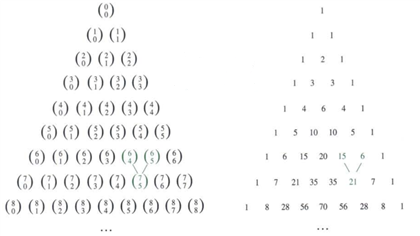
\includegraphics[scale=.8]{img/Pascal.png}
\end{center}
This is called Pascal's Triangle. Notice that each entry is the sum of the two diagonally above:
\begin{equation*}
\begin{split}
\mathtt{C}(n,r) &= \mathtt{C}(n-1,r-1) + \mathtt{C}(n-1,r) \\
{n \choose r} &= {n-1 \choose r-1} + {n-1 \choose r}
\end{split}
\end{equation*}
It is easy to show that this is correct algebraically:
\begin{equation*}
{n \choose r} = \frac{(n-1)!}{(n-r)!(r-1)!} + \frac{(n-1)!}{(n-r-1)!r!} = \frac{(n-1)!}{(n-r-1)!(r-1)!} \Big[ \frac{1}{n-r} + \frac{1}{r} \Big] = \frac{n!}{(n-r)!r!}
\end{equation*}

\end{itemize}
\end{lemma}
\end{minipage}}
\end{center}

\begin{example}
How many ways can a 5 card hand be selected from a deck of 52 distinct cards?
\end{example}
\begin{solution}
Since order does not matter:
\begin{equation*}
\mathtt{C}(52,5) = {52 \choose 5} = \frac{52!}{47!5!} = 2,598,960 \hspace{.1cm} \text{ways}
\end{equation*}
\end{solution}

\newpage
\begin{example}
Consider a group of $n$ distinct objects, $a_1,a_2,\dots,a_n$.
\begin{itemize}

\item[(a)]
How many distinct $r$-combinations are there?

\vspace{.2cm}
\item[(b)]
How many $r$-combinations include $a_1$?

\vspace{.2cm}
\item[(c)]
How many $r$-combinations exclude $a_1$?

\end{itemize}
\end{example}
\begin{solution}
\hfill
\begin{itemize}

\item[(a)]
Clearly, by definition, $\mathtt{C}(n,r) = {n \choose r} = \frac{n!}{(n-r)!r!}$. Notice that each selection of $r$ objects leaves behind a group of $n-r$ objects. Therefore, $\mathtt{C}(n,r) = \mathtt{C}(n,n-r)$. This is exactly the first observation made on the binomial coefficient.

\vspace{.2cm}
\item[(b)]
Since order does not matter, select $a_1$, and then all $(r-1)$-combinations from the $(n-1)$ objects $a_2,a_3,\dots,a_n$. Therefore, there are $\mathtt{C}(n-1,r-1)$ $r$-combinations that include $a_1$.

\vspace{.2cm}
\item[(c)]
These are found by picking $r$ objects from the $(n-1)$ objects $a_2,a_3,\dots,a_n$. Therefore, there are $\mathtt{C}(n-1,r)$ $r$-combinations that exclude $a_1$.

\end{itemize}
\end{solution}

\noindent
Notice that parts (b) and (c) are exclusive and represent all $r$-combinations: $\mathtt{C}(n,r) = \mathtt{C}(n-1,r-1) + \mathtt{C}(n-1,r)$. This is exactly the second observation made about the binomial coefficient.

\begin{example}
\hfill
\begin{itemize}

\item[(a)]
How many ways can a committee of 3 Republicans and 4 Democrats be chosen from a legislature which consists of 9 Republicans and 6 Democrats?

\vspace{.2cm}
\item[(b)]
How many ways can a committee of 3 Republicans and 4 Democrats be chosen if Republican Mr.A refuses to serve given that Democrat Mr.B is on the committee?

\end{itemize}
\end{example}
\begin{solution}
\hfill
\begin{itemize}

\item[(a)]
Let $R$ and $D$ represents the number of ways of picking out Republicans and Democrats respectively:
\begin{equation*}
\begin{split}
R &= {9 \choose 3} = 84 \hspace{.1cm} \text{ways} \\
D &= {6 \choose 4} = 15 \hspace{.1cm} \text{ways}
\end{split}
\end{equation*}
The total number of choices for a committee is given by: $(R \cap D) = 84 \times 15 = 1260$ ways.

\vspace{.2cm}
\item[(b)]
Could be split into mutually exclusive cases:
\begin{itemize}

\vspace{.2cm}
\item[(i)]
Committees with neither A nor B: Out of the 8 Republicans omitting Mr.A, pick 3 and out of the 5 Democrats omitting Mr.B, pick 4: ${8 \choose 3} {5 \choose 4} = 280$ ways.

\vspace{.2cm}
\item[(ii)]
Committees with A but not B: Similarly, we find: ${8 \choose 2} {5 \choose 4} = 140$ ways.

\vspace{.2cm}
\item[(iii)]
Committees with B but not A: Similarly, we find: ${8 \choose 3} {5 \choose 3} = 560$ ways.

\end{itemize}
\vspace{.2cm}
The total number of choices for a committee is given by: $280+140+560 = 980$ ways. A cleaner way of doing this is to count the committees with both A and B: ${8 \choose 2} {5 \choose 3} = 280$ ways and omit them from the total: $1260 - 280 = 980$ ways.

\end{itemize}
\end{solution}

\newpage
\section{\textbf{\underline{Selections and Arrangements with Repetition}}}
\vspace{.3cm}
\noindent
Consider counting the permutations in a case where some objects are not distinct:

\begin{example}
How many permutations are there of the 7 letters in the word GOGGLES? 
\end{example}
\begin{solution}
First imagine putting subscripts on the 3 G's, such as $G_1, G_2,$ and $G_3$. All 7 letters are now distinct, so there are 7! permutations with subscripts. Now consider the G's. If one of the permutations is given by $G_1OOG_2G_3LES$ and another as $G_2OOG_1G_3LES$, they are the same since the G's realistically are the same after removing the subscripts. Since the G's can be shuffled 3! ways, the total number of permutations accounting for the indistinguishable G's is $\frac{7!}{3!} = 840$ ways.
\end{solution}

\begin{center}
\fbox{
\begin{minipage}{7.3 in}
\begin{definition}[Permutations with Repetition]
In general, the number of $n$-permutations of $n$ objects, where there are $k_1$ of the $1^{st}$ kind, $k_2$ of the $2^{nd}$ kind, $\dots$, and $k_m$ of the $m^{th}$ kind, where $k_1+k_2+k_3+\dots+k_m=n$ is:
\begin{equation*}
\mathtt{P}(n;k_1,k_2,k_3,\dots,k_m) = \frac{n!}{k_1!k_2!k_3!\dots k_m!} = {n \choose k_1,k_2,k_3,\dots,k_m}
\end{equation*}
where ${n \choose k_1,k_2,k_3,\dots,k_m}$ is known as the multinomial coefficient.
\end{definition}
\end{minipage}}
\end{center}

\begin{example}
How many arrangements of GOGGLES start with a G?
\end{example}
\begin{solution}
Make the first letter a particular G. This leaves 6 letters for the remaining 6 positions, with one pair of G's. Thus:
\begin{equation*}
\mathtt{P}(6;2,1,1,1,1) = \frac{6!}{2!(1!)^4} = 360 \hspace{.1cm} \text{ways}
\end{equation*}
\end{solution}

\begin{example}
How many 3-permutations are there of the letters $a,a,a,b,c$?
\end{example}
\begin{solution}
No simple formula for this setup. Break into exclusive pieces: [a,a,a] or [a,a,b] or [a,a,c] or [a,b,c]. The total is therefore given by: $\frac{3!}{3!} + \frac{3!}{2!} + \frac{3!}{2!} + 3! = 13$ ways.
\end{solution}

\noindent
Consider next combinations with repeated objects:

\begin{example}[The Ice-Cream Problem]
How many $r=3$ scoop banana splits can be ordered if $n=6$ kinds of ice cream are available, and the scoops need not be different flavors?
\end{example}
\begin{solution}
Consider 3 cases:
\begin{itemize}

\vspace{.2cm}
\item[(i)]
3 Scoops the Same: Choose 3! ways

\vspace{.2cm}
\item[(ii)]
2 Scoops of 1 Flavor and 1 Scoop of Another Flavor: $6 \times 5 = 30$ ways

\vspace{.2cm}
\item[(iii)]
All 3 Flavors Different: $\mathtt{C}(6,3) = 20$ ways

\end{itemize}
The cases are mutually exclusive giving a total of $6+30+20 = 56$ ways. 
\end{solution}

\noindent
While the solution above is correct, it is too laborious for large problems. We therefore devise a better scheme:

\begin{center}
\fbox{
\begin{minipage}{7.3 in}
\begin{definition}[Dots \& Bars Model]
Use Example 6.4 as inspiration for this model. To generalize say there are $n$ flavors and $r$ scoops. Now imagine drawing $n-1$ parallel lines that have regions to the left and right of them that will represent the different $n$ flavors. Let black dots represent the $r$ scoops. Now to find the number of ways of permuting $(n-1)+(r)$ objects with each repeating $(n-1)$ and $r$ times respectively:
\begin{equation*}
\mathtt{P}(n+r-1;n-1,r) = \frac{(n+r-1)!}{(n-1)!r!} = {n+r-1 \choose r} = \mathtt{C}(n+r-1,r)
\end{equation*}
\end{definition}
\end{minipage}}
\end{center}

\begin{example}
How many ways are there to select 12 donuts from 5 different kinds if at least 5 must be sugar coated?
\end{example}

\newpage
\begin{solution}
Let $n=5$ represent the kinds and $r=12-5=7$ donuts since 5 must already be sugar coated no matter what. Using the dots and bars model:
\begin{equation*}
{11 \choose 4} = \frac{11!}{7!4!} = 33 \hspace{.1cm} \text{ways}
\end{equation*}
\end{solution}


\begin{example}
How many different ways are there to select 7 out of the first 25 numbers, $(1,2,3,\dots,25)$, such that no two chosen numbers are consecutive.
\end{example}
\begin{solution}
Imagine writing out the 25 numbers in serial order, then place bars under 7 to select them, and dots under the remaining 18 to leave them unselected. Setup the dots and bars to satisfy the restriction of no consectuive numbers being selected: Draw out 7 bars and place 6 dots to fill all the spaces in between. This leaves 12 dots to freely distribute before, between, and after giving:
\begin{equation*}
{19 \choose 12} = \frac{19!}{12!7!} \hspace{.1cm} \text{ways}
\end{equation*}
\end{solution}

\begin{example}
How many ways are there to form a sequence of 10 letters from an unlimited supply of a's, b's, c's, and d's, if each letter must appear at least twice?
\end{example}
\begin{solution}
Split into exclusive cases. Note that we use up 8 of 10 choices of letters satisfying the restriction that each letter appear twice. For the last 2 letters:
\begin{itemize}

\vspace{.2cm}
\item[(i)]
2 Different Letters: 4 ways to choose the last two letters. For the number of arrangements there are going to be 4 of one letter and 2 of all the other letters giving:
\begin{equation*}
\mathtt{P}(10;4,2,2,2) = \frac{10!}{4!(2!)^3} \hspace{.1cm} \text{ways}
\end{equation*}

\vspace{.2cm}
\item[(ii)]
Both the Same Letter: ${4 \choose 2} = 6$ ways to choose the last two letters. For the number of arrangements there are going to be 3 of two letters and 2 of the other two letters giving:
\begin{equation*}
\mathtt{P}(10;3,3,2,2) = \frac{10!}{(3!)^2(2!)^2} \hspace{.1cm} \text{ways}
\end{equation*}

\end{itemize}
The total number of ways is given by the sum of the exclusive cases:
\begin{equation*}
\mathtt{C}(4,1)\mathtt{P}(10;4,2,2,2) + \mathtt{C}(4,2)\mathtt{P}(10;3,3,2,2) = 4 \times \frac{10!}{4!(2!)^3} + 6 \times \frac{10!}{(3!)^2(2!)^2} = \frac{10!}{3!(2!)^3} + \frac{10!}{3!(2!)^2} = \frac{10!}{2^4} \hspace{.1cm} \text{ways}
\end{equation*}
\end{solution}

\vspace{.3cm}
\section{\textbf{\underline{Distributions}}}
\vspace{.3cm}
\noindent
In general, distribution of distinct objects correspond with arrangements and distributions of identical objects correspond with selection:

\begin{center}
\fbox{
\begin{minipage}{7.3 in}
\begin{definition}[Two Models of Distributions]
\hfill
\begin{itemize}

\item[(i)]
Distinct Objects Model: Distributing $r$ distinct objects into $n$ different (distinct) boxes without restrictions amounts to stamping one of the $n$ box numbers on each of the $r$ objects:
\begin{equation*}
\underbrace{(n)(n)(n) \dots (n)}_{r \hspace{.1cm} times} = n^r \hspace{.1cm} \text{distributions}
\end{equation*}

\item[(ii)]
Identical Objects Model: Distributing $r$ identical objects into $n$ different (distinct) boxes without restrictions amounts to selecting all $r$-subsets with repetition from the $n$ distinct boxes, which from the dots and bars model is the same as free distribution of $r$ dots into the $n$ boxes defined by $n-1$ bars:
\begin{equation*}
\mathtt{P}(n+r-1;n-1,r) = \mathtt{C}(n+r-1,r) = \frac{(n+r-1)!}{(n-1)!r!} \hspace{.1cm} \text{distributions}
\end{equation*}

\end{itemize}
\end{definition}
\end{minipage}}
\end{center}

\newpage
\begin{example}
\hfill
\begin{itemize}

\item[(a)]
How many ways can 20 students be sent to any 1 of 5 different advisers?

\item[(b)]
How many ways if each adviser must end up seeing just 4 students?

\end{itemize}

\end{example}
\begin{solution}
\hfill
\begin{itemize}

\item[(a)]
The first student can be sent to any of 5 advisers, so can the second, $\dots$:
\begin{equation*}
\underbrace{(5)(5)(5) \dots (5)}_{20 \hspace{.1cm} terms} = 5^{20} \hspace{.1cm} \text{ways}
\end{equation*}

\vspace{.2cm}
\item[(ii)]
Imagine lining students up in particular order. Call the advisers A, B, C, D, and E. The solution amounts to all arrangements of 4 A's, 4 B's, $\dots$, 4 E's under the 20 students giving:
\begin{equation*}
\mathtt{P}(20;4,4,4,4,4) = \frac{20!}{(4!)^5} \hspace{.1cm} \text{ways}
\end{equation*}

\end{itemize}
\end{solution}

\begin{example}
How many ways are there to distribute $r$ similar balls into $n$ numbered boxes if there must be at least one ball in each box? (Assume $r > n$)
\end{example}
\begin{solution}
Use the dots and bars model: Draw $n-1$ bars to define the $n$ boxes and put a dot in all the $n$ regions created by the $n-1$ bars. This uses $n$ of the $r$ dots available, thereby leaving $(r-n)$ dots. Finally, freely distribute the $(r-n)$ dots into the $n$ boxes in all ways:
\begin{equation*}
\mathtt{P}(r-1;r-n,n-1) = \frac{(r-1)!}{(r-n)!(n-1)!} \hspace{.1cm} \text{ways}
\end{equation*}
\end{solution}

\begin{example}
How many ways can the letters a, e, i, o, u, and 8 x's be arranged if no two vowels may be adjacent?
\end{example}
\begin{solution}
First consider the 5 vowels. These may be arranged in $5!=120$ ways. For each arrangement, consider the possible distribution of the 8 x's. Indicate the position of the 5 vowels with 5 bars (which define 6 boxes) and place dots between each pair of bars to indicate the locations of the x's which satisfies the restriction that vowels not be adjacent. Next freely distribute the remaining 4 dots before, between, and after the 5 bars: 
\begin{equation*}
\mathtt{P}(9;4,5) = \frac{9!}{4!5!} = 126 \hspace{.1cm} \text{ways}
\end{equation*}
Since this holds for each vowel arrangements, the solution is: $120 \times 126 = 15,120$ ways.
\end{solution}

\begin{example}
\hfill
\begin{itemize}

\item[(a)]
How many integer solutions are there to the equation: $x_1 + x_2 + x_3 + x_4 + x_5 + x_6 = 3$? (Assume $x_i \geq 0 \hspace{.1cm} \forall i \in \mathbb{N}$)

\vspace{.2cm}
\item[(b)]
More generally, how many integer solutions are there to: $x_1 + x_2 + \dots + x_n = r$? (Assume $x_i \geq 0 \hspace{.1cm} \forall i \in \mathbb{N}$)

\vspace{.2cm}
\item[(c)]
How many integer solutions are there to: $x_1 + x_2 + \dots + x_n = r$? (Assume $x_i > 0 \hspace{.1cm} \forall i \in \mathbb{N}$)

\end{itemize}
\end{example}

\newpage
\begin{solution}
\hfill
\begin{itemize}

\item[(a)]
Typically, a solution looks like: $x_1=1, x_2=0, x_3=0, x_4=2, x_5=0, x_6=0 \leftrightarrow (1,0,0,2,0,0)$. This is the same as having 3 dots, two of which lie in the $x_4$ box and 1 in the $x_1$ box. With 5 bars and 3 dots:
\begin{equation*}
\mathtt{P}(8;3,5) = \frac{8!}{3!5!} = 56 \hspace{.1cm} \text{ways}
\end{equation*}

\vspace{.2cm}
\item[(b)]
This is the same as putting $r$ identical balls into $n$ numbered boxes without restriction:
\begin{equation*}
\mathtt{P}(n+r-1;n-1,r) = \frac{(n+r-1)!}{(n-1)!r!} \hspace{.1cm} \text{ways}
\end{equation*}

\vspace{.2cm}
\item[(c)]
Clearly, $r \geq n$, and the problem is the same as putting $r$ identical balls into $n$ numbered boxes with at least one ball in each box:
\begin{equation*}
\mathtt{P}(r-1;n-1,r-n) = \frac{(r-1)!}{(r-n)!(n-1)!} \hspace{.1cm} \text{ways}
\end{equation*}

\end{itemize}
\end{solution}

\vspace{.2cm}
\noindent
It should by now be apparent that 3 seemingly different problems have the same solution:
\begin{itemize}

\vspace{.2cm}
\item[(1)]
Number of ways to select $r$ objects with repetition from $n$ types of objects

\vspace{.2cm}
\item[(2)]
Number of ways to distribute $r$ identical objects into $n$ distinct boxes

\vspace{.2cm}
\item[(3)]
Number of non-negative integer solutions to: $x_1 + x_2 + x_3 + \dots + x_n = r$

\end{itemize}

\begin{example}
\hfill
\begin{itemize}

\item[(a)]
How many ways are there to distribute 4 identical and 6 distinct objects into 5 distinct boxes?

\vspace{.2cm}
\item[(b)]
What if each box must contain 2 objects?

\end{itemize}
\end{example}
\begin{solution}
\hfill
\begin{itemize}

\item[(a)]
Treat the object separately. For the 4 identical objects and 5 distinct boxes use the dots and bars model:
\begin{equation*}
\mathtt{P}(8;4,4) = \frac{8!}{(4!)^2} = 70 \hspace{.1cm} \text{ways}
\end{equation*}
For the 6 distinct objects and 5 distinct boxes: $(5)(5)(5)(5)(5)(5) = 5^6 = 15,625$ ways. Since the cases are disjoint, the total numbers of way is given by: $(70)(15,625) = 1,093,750$ ways.

\vspace{.2cm}
\item[(b)]
Split into cases depending upon how the identical objects are distributed:
\begin{itemize}

\vspace{.2cm}
\item[(i)]
2 identical objects in each of 2 boxes: Pick the 2 boxes for identical objects from the 5 in ${5 \choose 2} = 10$ ways, then distribute the distinct objects into the 3 remaining boxes, 2 to a box, in $\mathtt{P}(6;2,2,2) = \frac{6!}{(2!)^3} = 90$ ways. The total number of ways is given by $(10)(90) = 900$ ways.

\vspace{.2cm}
\item[(ii)]
2 identical objects in one box, and one identical object in each of 2 boxes: First, pick a box to get the 2 identical objects in ${5 \choose 1} = 5$ ways, then pick two more boxes each to get one identical object in ${4 \choose 2} = 6$ ways. The 6 distinct objects can then be distributed in $\mathtt{P}(6;2,2,1,1) = \frac{6!}{(2!)^2(1!)^2} = 180$ ways. The total number of ways is given by $(5)(6)(180) = 5,400$ ways.

\vspace{.2cm}
\item[(iii)]
1 identical object in each of 4 boxes: Pick the 4 boxes in ${5 \choose 4} = 5$ ways, then distribute the 6 distinct objects in $\mathtt{P}(6;2,1,1,1,1) = \frac{6!}{2!(1!)^4} = 360$ ways. The total number of ways is given by $(5)(360) = 1,800$ ways.

\end{itemize}
Since each case is exclusive the total number of ways is defined as: $900 + 5,400 + 1,800 = 8,100$ ways.

\end{itemize}
\end{solution}

\noindent
If we wanted to calculate the probability that each box would contain 2 objects, would have to proceed with care as our present cases are not all equally likely.

\newpage
\section{\textbf{\underline{Applications of Combinatorics to Probability}}}
\vspace{.3cm}
\noindent
We look now at applications of combinatorial methods to finding probabilities using Laplace's definition of probability:

\begin{example}
\hfill
\begin{itemize}

\item[(a)]
What is the probability of getting at least one "6" in $r$ rolls of a "fair" die?

\vspace{.2cm}
\item[(b)]
What is the least number of people, $r$, required such that at least one has the same birthday as you with a probability of at least $\frac{1}{2}$?

\vspace{.2cm}
\item[(c)]
What is the least number of people, $r$, required such that the probability that two or more share the same birthday with a probability of at least $\frac{1}{2}$

\end{itemize}
\end{example}
\begin{solution}
\hfill
\begin{itemize}

\item[(a)]
Let A = event of getting no "6's" in $r$ rolls. Then A' = $A^\mathsf{c}$ = event of getting 1 or 2 or 3 or $\dots$ or $r$ "6's" in $r$ rolls. Using this setup gives:
\begin{equation*}
\mathbb{P}[A] + \mathbb{P}[A'] = 1 \implies \mathbb{P}[A'] = 1 - \mathbb{P}[A] = 1 - \frac{\underbrace{(5)(5)\dots (5)}_{r \hspace{.1cm} terms}}{\underbrace{(6)(6)\dots (6)}_{r \hspace{.1cm} terms}} = 1 - \Big( \frac{5}{6} \Big)^r
\end{equation*}

\vspace{.2cm}
\item[(b)]
Visualize this as rolling a 365 sided fair die with the number 1 being your birthday. Following the argument form part (a), we conclude that:
\begin{equation*}
1 - \Big( \frac{364}{365} \Big)^r > \frac{1}{2} \implies r \geq 253
\end{equation*}

\vspace{.2cm}
\item[(c)]
Let $\mathbb{P}[$No Common Birthday$] = \frac{m}{n}$ where $n$ = total arrangements of $r$ birthday = $(365)^r$ and $m$ = total arrangements of $r$ different birthdays = $\mathtt{P}(365,r) = \frac{365!}{(365-r)!}$. Using this setup gives:
\begin{equation*}
\mathbb{P}[\text{At Least 1 Common Birthday}] = 1 - \frac{m}{n} = 1 - \frac{365!}{(365-r)!(365)^r} > \frac{1}{2} \implies r \geq 23
\end{equation*}

\end{itemize}
\end{solution}

\begin{example}
Six identical balls are distributed randomly into 3 distinct boxes. What is the probability that all boxes are occupied?
\end{example}
\begin{solution}
Imagine balls to be distinct, this will make all cases equally likely. First, find $n$, the number of ways boxes can be filled. Each ball can go into any of the 3 boxes $(3)(3)(3)(3)(3)(3) = 3^6 = 729$ ways. If no box is left empty, balls can be distributed in 3 distinct ways:
\begin{itemize}

\vspace{.2cm}
\item[(i)]
2 balls in each box: Imagine lining balls up in serial order and distributing 2 "1's", 2 "2's", and 2 "3's" beneath to indicate which box balls go into $\mathtt{P}(6;2,2,2) = \frac{6!}{(2!)^3} = 90$ ways.

\vspace{.2cm}
\item[(ii)]
3,2, and 1 ball(s), respectively, in the 3 boxes: Similar argument to part(i) $\rightarrow \mathtt{P}(6;3,2,1) = 60$ ways. Then we must decide which box gets 3 balls, which gets 2, and the remaining box gets 1. Pick a box to get 3 balls in ${3 \choose 1} = 3$ ways and then pick a box to get 2 balls in ${2 \choose 1} = 2$ ways giving a total number of $(60)(3)(2) = 360$ ways.

\vspace{.2cm}
\item[(iii)]
4 balls in one box, and 1 in each of the other 2 boxes: As in part (i) $\rightarrow \mathtt{P}(6;4,1,1) = 30$ ways. Then decide which box gets 4 balls in ${3 \choose 1} = 3$ ways giving a total number of $(30)(3) = 90$ ways.

\end{itemize}
The total number of ways to have at least one ball in each box is $m=90+360+90=540$ ways. Therefore:
\begin{equation*}
\mathbb{P}[\text{All Boxes Occupied}] = \frac{m}{n} = \frac{540}{729} = \frac{20}{27}
\end{equation*}
\end{solution}

\noindent
If the boxes had been identical, would have imagined numbering them also. The result would still have been $\frac{20}{27}$.

\newpage
\begin{example}
\hfill
\begin{itemize}

\item[(a)]
Six cards are drawn from an ordinary deck. What is the probability of exactly one pair?

\vspace{.2cm}
\item[(b)]
What would be the probability of two pairs?

\end{itemize}
\end{example}
\begin{solution}
\hfill
\begin{itemize}

\item[(a)]
First consider the pair. First card can be any of 52, its match can then be any of 3, thus there are $(52)(3)$ 2-permutations of matching cards. Since order is irrelevant, divide by 2! $\rightarrow \frac{(52)(3)}{2!}$. Next consider the four unpaired cards. First can be any of 48, second any of 44, etc... $\rightarrow (48)(44)(40)(36)$. Once again this counts the 4-permutations, so divide by $4!$ giving a the total number of ways of getting a favorable hand: $\frac{(52)(3)(48)(44)(40)(36)}{2!4!}$. Therefore, the probability is defined as:
\begin{equation*}
\mathbb{P}[\text{Exactly 1 Pair}] = \frac{\frac{(52)(3)(48)(44)(40)(36)}{2!4!}}{{52 \choose 6}} = \frac{6!46!(52)(3)(48)(44)(40)(36)}{2!4!52!}
\end{equation*}

\vspace{.2cm}
\item[(b)]
Could use the above procedure, but will instead illustrate another. Consider first face value, then suit. Since there are 13 different face values, choose 2 for pairs in ${13 \choose 2}$ ways. This leaves 11 out of which choose 2 singles in ${11 \choose 2}$ ways. Next consider the suit. For each pair choose 2 out of the four suits in ${4 \choose 2}^2$ ways for both pairs. Also choose a suit for each single in ${4 \choose 1}^2$ ways for both singles. Therefore, the probability is defined as:
\begin{equation*}
\mathbb{P}[\text{Exactly 2 Pairs}] = \frac{{13 \choose 2}{4 \choose 2}^2 {11 \choose 2}{4 \choose 1}^2}{{52 \choose 6}}
\end{equation*}

\end{itemize}
\end{solution}

\begin{example}
Consider 5 card stud poker:
\begin{itemize}

\vspace{.2cm}
\item[(a)]
What is the probability of getting a straight flush (5 cards in order and of the same suit)?

\vspace{.2cm}
\item[(b)]
What is the probability of getting a flush?

\vspace{.2cm}
\item[(c)]
What is the probability of getting a straight?

\vspace{.2cm}
\item[(d)]
What is the probability of getting nothing?

\end{itemize}
\end{example}
\begin{solution}
\hfill
\begin{itemize}

\item[(a)]
Total possible number of hands: ${52 \choose 5}$. Straight Flushes: 10 straights/suit (1,2,3,4,5; 2,3,4,5,6; $\dots$; 10,J,Q,K,1) $\times$ 4 suits = 40 Straight Flushes. Therefore, $\mathbb{P}[\text{Straight Flush}] = \frac{40}{{52 \choose 5}} = \frac{40}{2,598,960}$.

\vspace{.2cm}
\item[(b)]
Total possible number of hands: ${52 \choose 5}$. Flush: 5 Cards in one suit ${13 \choose 5} \times$ 4 suits = 5,148 Flushes. Therefore, $\mathbb{P}[\text{Flush}] = \frac{5,148}{{52 \choose 5}} = \frac{5,148}{2,598,960}$.

\vspace{.2cm}
\item[(c)]
As above, there are 10 different straights ignoring suit. Each of the 5 cards can be any 4 suits giving a total of $10 \times (4)^5$ straights. Therefore, $\mathbb{P}[\text{Straight}] = \frac{10\times (4)^5}{{52 \choose 5}} = \frac{10,240}{2,598,960}$.

\vspace{.2cm}
\item[(d)]
Disregarding suit, there are ${13 \choose 5}$ hands with 5 different face values, but 10 of these are straights giving $\Big[ {13 \choose 5} - 10 \Big]$ that would give nothing. Now to consider the suit, each of the 5 cards can be any of four suits, thus there are $4^5$ combinations, but 4 of these would be flushes giving $\Big[ 4^5 - 4 \Big]$ that would give nothing. Hence the probability of a nothing hand is:
\begin{equation*}
\mathbb{P}[\text{Nothing}] = \frac{\Big[ {13 \choose 5} - 10 \Big] \Big[ 4^5 - 4 \Big]}{{52 \choose 5}} = \frac{1,302,540}{2,598,960} \approx .501
\end{equation*}

\end{itemize}
\end{solution}

\noindent
This last calculation helps explain why poker is a good game. Roughly half the time one would expect to get a pair or better.

\newpage
\section{\textbf{\underline{The Binomial Theorem}}}
\vspace{.3cm}
\noindent
Consider the expansion:
\begin{equation*}
(x_1+y_1)(x_2+y_2) = x_1x_2 + x_1y_2 + y_1x_2 + y_1y_2
\end{equation*}
Since each term on the right contains an entry with a subscript 1 and an entry with subscript 2, each term contains an entry from within each parenthesis. Now let $x_1=x_2=x$ and $y_1=y_2=y$:
\begin{equation*}
(x+y)(x+y) = (x+y)^2 = x^2 + 2xy + y^2
\end{equation*}
Terms arise as above, but some are identical to others and can be grouped. To generalize:
\begin{equation*}
(x_1+y_1)(x_2+y_2)\dots(x_n+y_n) = x_1x_2\dots x_n + \dots
\end{equation*}
How many terms will there be? Since each results from selecting one of the 2 terms within each of pair of parenthesis gives $\underbrace{(2)(2)(2)\dots(2)}_{\text{n terms}} = 2^n$. Next let $x_1=x_2=\dots=x_n=x$ and $y_1=y_2=\dots=y_n=y$:
\begin{equation*}
(x+y)^n = \Big( \hspace{.2cm} \Big) x^n + \Big( \hspace{.2cm} \Big) x^{n-1} y + \Big( \hspace{.2cm} \Big) x^{n-2} y^2 + \dots + \Big( \hspace{.2cm} \Big) x^{n-r} y^r + \dots + \Big( \hspace{.2cm} \Big) y^n
\end{equation*}
What should the coefficients be on the grouped terms? Consider the general term $x^{n-r} y^r \hspace{.1cm} \forall r \in \mathbb{Z}^*$ \footnotemark. There are $n+1$ terms in all. All terms that are counted in $x^{n-r} y^r$ result from having $(n-r)$ parenthesis contribute a $x$, and the remaining $r$ parenthesis contribute a $y$. The coefficient is ${n \choose r} = {n \choose n-r}$ giving:

\begin{center}
\fbox{
\begin{minipage}{7.3 in}
\begin{definition}[The Binomial Theorem]
\begin{equation*}
(x+y)^n = {n \choose 0}x^n + {n \choose 1}x^{n-1}y + {n \choose 2}x^{n-2}y^2 + \dots {n \choose r}x^{n-r}y^r + \dots + {n \choose n}y^n = \sum_{r=0}^n {n \choose r} x^{n-r} y^r \hspace{.3cm} \forall n \in \mathbb{Z}^*
\end{equation*}
This expression is called the Binomial Series or Binomial Theorem. It follows easily that:
\begin{itemize}

\item[(1)]
If $x=1$ and $y=\zeta$:
\begin{equation*}
(1+\zeta)^n = \sum_{r=0}^n {n \choose r}\zeta^r
\end{equation*}

\item[(2)]
If $x=1$ and $y=-\zeta$:
\begin{equation*}
(1-\zeta)^n = \sum_{r=0}^n {n \choose r}(-\zeta)^r = \sum_{r=0}^n (-1)^r {n \choose r}\zeta^r
\end{equation*}

\end{itemize}
\end{definition}
\end{minipage}}
\end{center}

\begin{example}
Find the coefficient of $a^{12}b^7$ in the expansion of $(6a-5b)^{19}$.
\end{example}
\begin{solution}
Let $x=6a$, $y=-5b$, and $n=19$:
\begin{equation*}
(6a-5b)^{19} = \sum_{r=0}^{19} {19 \choose r} (6a)^{19-r} (-5b)^r
\end{equation*}
Thus, if $r=7$ the term is ${19 \choose 7} (6a)^{12} (-5b)^7$ giving a coefficient of $-{19 \choose 7} 6^{12} 5^7$.
\end{solution}

\begin{center}
\fbox{
\begin{minipage}{7.3 in}
\begin{lemma}[Known Properties of the Binomial Coefficient]
\hfill
\begin{itemize}

\item[(1)]
\begin{equation*}
{n \choose r} = \frac{n!}{(n-r)!r!} = {n \choose n-r}
\end{equation*}

\item[(2)]
\begin{equation*}
{n \choose r} = {n-1 \choose r-1} + {n-1 \choose r}
\end{equation*}

\end{itemize}
\end{lemma}
\end{minipage}}
\end{center}

\footnotetext{$\mathbb{Z}^* = \{ 0 \} \cup \mathbb{Z}^+ = $ set of non-negative integers}

\newpage
\begin{center}
\fbox{
\begin{minipage}{7.3 in}
\begin{lemma}[Property of the Binomial Coefficient]
Another useful relationship for the binomial coefficient is:
\begin{equation*}
{n \choose k}{m \choose k} = {n \choose k}{n-k \choose m-k}
\end{equation*}
Although this is easy to show algebraically, consider the following combinatorial method:
\begin{proof}
Out of $n$ people select a group of size $m$ and then pick $k$ of these $m$ people to be a group of leaders. This is the same as first picking the $k$ leaders followed by picking out the remaining $m-k$ group members out of the $n-k$ non-leaders.
\end{proof}
\end{lemma}
\end{minipage}}
\end{center}


\begin{center}
\fbox{
\begin{minipage}{7.3 in}
\begin{definition}[Generalized Model for the Binomial Coefficient]
We now introduce a model which provides a useful visualization of many binomial identities. Consider a person walking on a street grid, starting from the top and progressing downward. 
\begin{center}
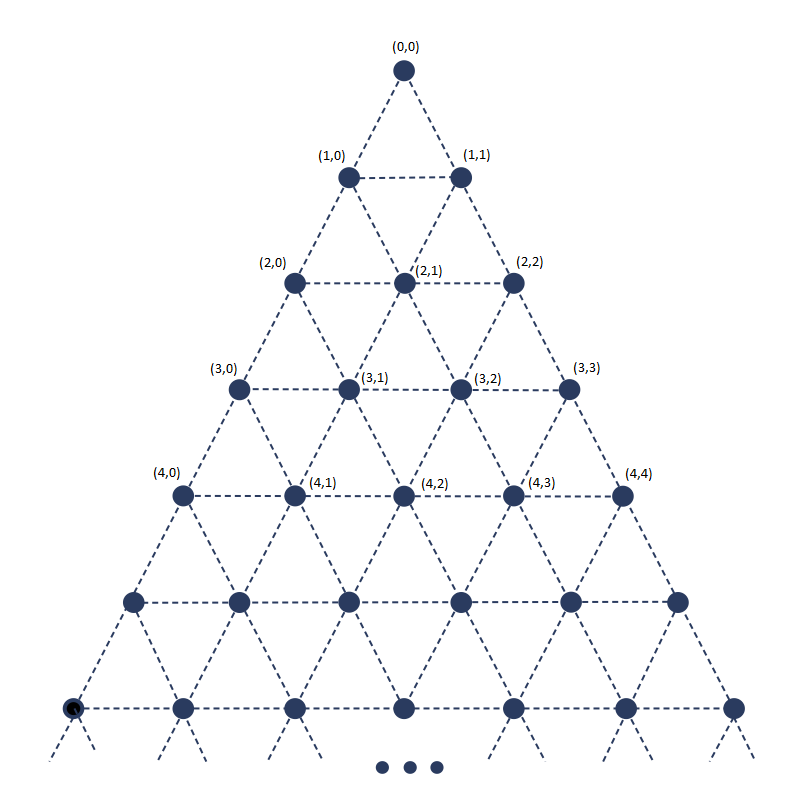
\includegraphics[scale=.2]{img/Generalized_Model.png}
\end{center}
At each intersection a person decides to go either left or right. The vertices (intersections) have been labeled in accordance with the number of total blocks and "right" decisions required to get a person to that point. Thus the vertex $(n,r)$ is $n$ blocks away from $(0,0)$ and required $r$ "right" decisions, and hence $(n-r)$ left decisions to get a person there. If we ask for the number of different paths from $(0,0)$ to $(n,r)$, the answer can be visualized in 2 ways:
\begin{itemize}

\vspace{.2cm}
\item[(i)]
At $r$ of the $n$ intersections, choose to go right, and hence go left at the other $(n-r)$ routes.

\vspace{.2cm}
\item[(ii)]
Count the number of possible $n$ letter "words" written with $r$ "R's" and $(n-r)$ "L's". Any such word tells a walker how to turn at each successive intersection giving $\mathtt{P}(n;n-r,r) = {n \choose r}$ routes.

\end{itemize}
\vspace{.3cm}
Now use this scheme to prove some identities. For example, recall the identity:
\begin{equation*}
{n \choose r} = {n-1 \choose r} + {n-1 \choose r-1}
\end{equation*}
\begin{center}
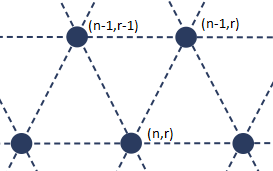
\includegraphics[scale=.2]{img/BC_Identity_Visualization.png}
\end{center}
\begin{proof}
To get to corner $(n,r)$ a walker must pass through either $(n-1,r-1)$ and go right or $(n-1,r)$ and go left. Since there is no other way, number of routes to $(n,r)$ is the sum of the numbers to $(n-1,r-1)$ and to $(n-1,r)$.
\end{proof}
Another useful identity is:
\begin{equation*}
{r \choose r} + {r+1 \choose r} + {r+2 \choose r} + \dots + {n \choose r} = {n+1 \choose r+1}
\end{equation*}
The first diagram illustrates the case with $r=1$ and $n=3$. Each route to $(4,2)$ can be decomposed into a route to each of the vertices on the left hand side of the equation, $(1,1), (2,1), (3,1)$, by right and then only left decisions. Since there is only one route to $(4,2)$ from the last vertex, this scheme proves the identity.
\end{definition}
\end{minipage}}
\end{center}

\newpage
\begin{center}
\fbox{
\begin{minipage}{7.3 in}
\begin{lemma}[Evaluating Identities]
Another method for evaluating identities follows directly from the Binomial Series:
\begin{equation*}
(1+\zeta)^n = \sum_{r=0}^n {n \choose r} \zeta^n
\end{equation*}
\begin{itemize}

\item[(1)]
Set $\zeta=1$:
\begin{equation*}
(1+1)^n = 2^n = \sum_{r=0}^n {n \choose r}
\end{equation*}

\item[(2)]
Set $\zeta=-1$:
\begin{equation*}
(1-1)^n = 0 = \sum_{r=0}^n (-1)^n {n \choose r}
\end{equation*}

\item[(3)]
Differentiate with respect to $\zeta$ and then set $\zeta=1$:
\begin{equation*}
\begin{split}
n(1+\zeta)^{n-1} = \sum_{r=1}^n r {n \choose r} \zeta^{r-1} \\
n(1+1)^{n-1} = n 2^{n-1} = \sum_{r=1}^n r {n \choose r}
\end{split}
\end{equation*}

\end{itemize}
\end{lemma}
\end{minipage}}
\end{center}

\begin{center}
\fbox{
\begin{minipage}{7.3 in}
\begin{definition}[Generalization of the Binomial Theorem]
Recall that:
\begin{equation*}
{n \choose r} = \frac{n!}{(n-r)!r!} = \frac{n(n-1)(n-2)\dots(n-r+1)}{r!} \hspace{.3cm} \forall n,r \in \mathbb{Z} \hspace{.3cm} \text{and} \hspace{.3cm} n \geq r
\end{equation*}
Formally, replace $n$ by $w$ where $w$ is any real number:
\begin{equation*}
{w \choose r} = \frac{w!}{(w-r)!r!} = \frac{w(w-1)(w-2)\dots(w-r+1)}{r!} \hspace{.3cm} \forall w \in \mathbb{R}, \hspace{.3cm} \forall r \in \mathbb{Z} \hspace{.3cm} \text{and} \hspace{.3cm} w \geq r
\end{equation*}
The Binomial Series then generalizes to:
\begin{equation*}
(1+\zeta)^w = \sum_{r=0}^\infty {w \choose r} \zeta^r
\end{equation*}
Note that the upper limit on the sum is now $\infty$. In fact, for any $w$ we could write this limit as $\infty$ since if $w=n$ all terms beyond $r=n$ have zero coefficients. Now for a generalized identity:
\begin{equation*}
\begin{split}
{-w \choose r} &= \frac{(-w)(-w-1)(-w-2)\dots(-w-r+1)}{r!} \\
&= (-1)^r \frac{(w+r-1)\dots(w+2)(w+1)(w)}{r!} \\
&= (-1)^r {w+r-1 \choose r} \hspace{.3cm} \forall w \in \mathbb{R}^+
\end{split}
\end{equation*}
This identity will be very useful when discussing generating functions.
\end{definition}
\end{minipage}}
\end{center}

\newpage
\section{\textbf{\underline{Generating Functions}}}
\vspace{.3cm}
\noindent
We now introduce an abstract concept called a generating function which will serve to unify prior results in combinatorics. Assume that $a_r$ is the number of ways to select $r$ objects subject to some set of restrictions. Then $g(x)$ is the generating function for $a_r$ if:
\begin{equation*}
g(x) = a_0 + a_1x + a_2x^2 + \dots + a_rx^r + \dots
\end{equation*}
If we can somehow encode the restrictions peculiar to a problem in the form of $g(x)$, then the answer is nothing more than the coefficient of $x^r$ in the polynomial form of $g(x)$. As an example recall from the section on the Binomial Theorem:
\begin{equation*}
(1+x)^n = {n \choose 0} + {n \choose 1}x + {n \choose 2}x^2 + \dots + {n \choose r}x^r + \dots + {n \choose n}x^n
\end{equation*}
Thus if $g(x) = (1+x)^n$, the coefficient of $x^r$ which represents $a_r$ is given by ${n \choose r}$. This particular choice of $g(x)$ caused us to find as a solution the number of $r$-combinations which can be selected from $n$ distinct objects. In general though, how do we write down the generating function? Note that for our purposes $x$ has no meaning other than as an encoding device, technically called an \textit{indicator variable}. In writing down the generating function we observe the following rules:
\begin{itemize}

\vspace{.2cm}
\item[(1)]
For each type of object available for selection write down a polynomial in $x$ with coefficients "1" and exponents equal to the number of times this object may be selected. For example, if we have only one object of a particular type, and if it may be either not selected (selected zero times) or selected (selected one time), then the appropriate term in the generating function is:
\begin{equation*}
(x^0 + x^1) \equiv 1 + x
\end{equation*}

\vspace{.2cm}
\item[(2)]
If we have an unlimited supply of a particular type of object, and we may choose any integer number of this type of object, the appropriate term in the generating function is:
\begin{equation*}
1 + x + x^2 + x^3 + \dots
\end{equation*}

\vspace{.2cm}
\item[(3)]
If we have 10 objects of a particular type and the restriction that we must select 2,4,6,8, or all 10, then the appropriate term in the generating function is:
\begin{equation*}
x^2 + x^4 + x^6 + x^8 + x^10
\end{equation*}

\end{itemize}
The generating function for a particular problem consists of a product of terms of the types listed, with one term for each type of object.

\begin{example}
Write down the generating function for the number of ways to select $r$ objects from a set consisting of $n$ distinct objects.
\end{example}
\begin{solution}
Since each object can either omitted or selected once, for each of the $n$ objects the appropriate expression is $(1+x)$. Thus:
\begin{equation*}
g(x) = \underbrace{(1+x)(1+x)\dots(1+x)}_{\text{n terms}} = (1+x)^n = \sum_{r=0}^n {n \choose r} x^r
\end{equation*}
Since we want to know the number of ways to select $r$ objects, the solution is the coefficient of $x^r$: ${n \choose r}$.
\end{solution}

\begin{example}
Write down a generating function for the number of integer solutions to:
\begin{equation*}
z_1 + z_2 + z_3 + z_4 = 14 \hspace{.3cm} \text{where} \hspace{.3cm} z_1 \geq 0, z_2 > 0, z_3 > 0, z > 0, \hspace{.3cm} z_3 \hspace{.3cm} \text{is odd and}, \hspace{.3cm} z_4 \hspace{.3cm} \text{is even}
\end{equation*}
\end{example}

\newpage
\begin{solution}
The contributions from each of the $z_i$ is:
\begin{equation*}
\begin{split}
g_{z_1}(x) &= 1 + x + x^2 + \dots + x^{14} \\
g_{z_2}(x) &= x + x^2 + x^3 + \dots + x^{14} \\
g_{z_3}(x) &= x + x^3 + x^5 + \dots + x^{13} \\
g_{z_4}(x) &= x^2 + x^4 + x^6 + \dots + x^{14}
\end{split}
\end{equation*}
which gives a generating function of:
\begin{equation*}
\begin{split}
g(x) &= g_{z_1}(x) g_{z_2}(x) g_{z_3}(x) g_{z_4}(x) \\
&= \Big( 1 + x + x^2 + \dots + x^{14} \Big) \Big( x + x^2 + x^3 + \dots + x^{14} \Big) \Big( x + x^3 + x^5 + \dots + x^{13} \Big) \Big( x^2 + x^4 + x^6 + \dots + x^{14} \Big)
\end{split}
\end{equation*}
To find the number of solutions to the given equation, determine the coefficient of $x^{14}$ in $g(x)$.
\end{solution}

\begin{example}
Write down the generating function for the number of ways to select $r$ balls from a set of balls consisting of 3 red, 3 black, 3 white, and 3 green balls.
\end{example}
\begin{solution}
The appropriate term for the red balls is:
\begin{equation*}
g_R(x) = 1 + x + x^2 + x^3
\end{equation*}
This is also the term for the black, white, and green balls giving:
\begin{equation*}
g(x) = g_R(x) g_B(x) g_W(x) g_G(x) = (1 + x + x^2 + x^3)^4
\end{equation*}
To find the number of ways to select $r$ balls from this particular set is given by the coefficient of $x^r$ in $g(x)$.
\end{solution}

\begin{center}
\fbox{
\begin{minipage}{7.3 in}
\begin{lemma}[Identities]
Before working out some examples, we note 3 useful identities:
\begin{itemize}

\item[(1)]
\begin{equation*}
1 + x + x^2 + x^3 + \dots = \frac{1}{1-x} \hspace{.3cm} \forall x \in (-1,1)
\end{equation*}

\item[(2)]
\begin{equation*}
1 + x + x^2 + \dots + x^r = \frac{1-x^{r+1}}{1-x}
\end{equation*}

\item[(3)]
\begin{equation*}
(1-x)^{-m} = \sum_{r=0}^\infty {-m \choose r} (-x)^r = \sum_{r=0}^\infty (-1)^r {r+m-1 \choose r} (-x)^r = \sum_{r=0}^\infty {r+m-1 \choose r} x^r
\end{equation*}

\end{itemize}
\end{lemma}
\end{minipage}}
\end{center}

\begin{example}[The Ice-Cream Problem Revisited]
How many 3 scoop banana splits can be made if 6 flavors of ice cream are available?
\end{example}
\begin{solution}
For each flavor, the appropriate term is:
\begin{equation*}
g_1(x) = 1 + x + x^2 + x^3 + \dots
\end{equation*}
Thus:
\begin{equation*}
g(x) = (g_1(x))^6 = (1 + x + x^2 + x^3 + \dots)^6 = (1-x)^{-6} = \sum_{r=0}^\infty {r+5 \choose r} x^r
\end{equation*}
The solution corresponds to the coefficient of $x^3$ which is ${8 \choose 3} = 56$ ways. For this setup one might say that since you can never select more than 3 scoops of any flavor, the generating function should take on a different form. Using the revised generating function, the coefficient of $x^3$ is still ${8 \choose 3} = 56$ ways:
\begin{equation*}
g(x) = (1 + x + x^2 + x^3)^6 = \Big[ \frac{1-x^4}{1-x} \Big]^6 = (1-x^4)^6 (1-x)^{-6} = (1 - 6x^4 + \dots) \sum_{r=0}^\infty {r+5 \choose 5} x^r
\end{equation*}
\end{solution}

\newpage
\begin{example}
Imagine that you are given 5 different kinds of objects. You have an unlimited supply of 3 of the types, but only one for each of the other 2 types.
\begin{itemize}

\vspace{.2cm}
\item[(a)]
Find the number of 3-combinations

\vspace{.2cm}
\item[(b)]
Find the number of 6-combinations

\end{itemize}
\end{example}
\begin{solution}
For each of the 3 types of objects which are available in unlimited supply:
\begin{equation*}
E_U(t) = 1 + t + t^2 + t^3 + \dots
\end{equation*}
For each of the 2 types of objects which there is only one of:
\begin{equation*}
E_1(t) = 1 + t
\end{equation*}
Thus the generating function is defined as:
\begin{equation*}
\begin{split}
E(t) &= (E_U(t))^3(E_1(t))^2 = (1 + t + t^2 + t^3 + \dots)(1 + t)^2 = \frac{(1+t)^2}{(1-t)^3} \\
&= (1 + 2t + t^2) \sum_{j=0}^\infty {-3 \choose j} (-t)^j \\
&= (1 + 2t + t^2) \sum_{j=0}^\infty {j+2 \choose j} t^j
\end{split}
\end{equation*}
\begin{itemize}

\vspace{.2cm}
\item[(a)]
From the generating function, the coefficient of $t^3$ is given by ${3 \choose 2} + 2{4 \choose 2} + {5 \choose 2} = 25$ 3-combinations.

\vspace{.2cm}
\item[(b)]
From the generating function, the coefficient of $t^6$ is given by ${6 \choose 2} + 2{7 \choose 2} + {8 \choose 2} = 85$ 6-combinations.

\end{itemize}
\end{solution}

\begin{example}
How many $r$-combinations are there out of $n$ distinct objects, if each object must appear at least once?
\end{example}
\begin{solution}
Each object has the term:
\begin{equation*}
E_i(t) = t + t^2 + t^3 + \dots
\end{equation*}
Thus the overall generating function is:
\begin{equation*}
\begin{split}
E(t) &= E_1(t)E_2(t)E_3(t)\dots E_n(t) = (t + t^2 + t^3 + \dots)^n \\
&= (t(1 + t + t^2 + t^3 \dots))^n = t^n (1 + t + t^2 + t^3 + \dots)^n \\
&= t^n (1-t)^{-n} = t^n \sum_{i=0}^\infty {n+i-1 \choose i} t^i \\
&= \sum{i=0}^\infty {n+i-1 \choose i} t^{n+i} = \sum_{r=n}^\infty {r-1 \choose r-n} t^r \\
&= \sum_{r=n}^\infty {r-1 \choose n-1} t^r
\end{split}
\end{equation*}
The number of $r$-combinations is given by the coefficient of series ${r-1 \choose n-1}$ if $r \geq n$ and 0 otherwise. Note that this is the same answer we found using the dots and bars model except that the roles of the $n$ and $r$ are interchanged. 
\end{solution}

\newpage
\begin{example}
Suppose we roll 4 distinguishable dice. How many ways can we have a sum of 17 appear?
\end{example}
\begin{solution}
For each die:
\begin{equation*}
E_D(t) = t + t^2 + t^3 + t^4 + t^5 + t^6
\end{equation*}
So for all 4 dice:
\begin{equation*}
\begin{split}
E(t) &= (E_D(t))^4 = (t + t^2 + t^3 + t^4 + t^5 + t^6)^4 \\
&= t^4 (1 + t + \dots + t^5)^4 = t^4 (1-t^6)^4 (1-t)^{-4} \\
&= t^4 (1 - 4t^6 + 6t^{12} - 4t^{18} + t^{24}) \sum_{j=0}^\infty {j+3 \choose j} t^j
\end{split}
\end{equation*}
The solution in this case is represented by the coefficient of $x^{17}$. An easier way is to find the solution is to determine the coefficient of $x^{13}$ in the following generating function:
\begin{equation*}
E^*(t) = \frac{E(t)}{t^4} = (1 - 4t^6 + 6t^{12} - 4t^{18} + t^{24}) \sum_{j=0}^\infty {j+3 \choose j} t^j
\end{equation*}
The coefficient of $x^{13}$ is given by ${16 \choose 13} - 4{10 \choose 7} + 6{4 \choose 1} = 104$ ways. If we were curious about the probability of the 4 dice having sum 17, it would be given by:
\begin{equation*}
\mathbb{P}[\text{sum} = 17] = \frac{104}{6^4} = \frac{104}{1296} = 0.08 = 8\%
\end{equation*}
\end{solution}

\begin{example}
In how many ways can $2n+1$ seats in a congress be distributed among 3 parties so that a coalition of any 2 parties will ensure a majority? 
\end{example}
\begin{solution}
If any 2 parties command a majority it means they have $n+1$ seats. Since no party alone has a majority and each party holds at least one seat, the appropriate term for each party is:
\begin{equation*}
E_i(t) = t + t^2 + t^3 + \dots + t^n
\end{equation*}
So for all 3 parties:
\begin{equation*}
E(t) = E_1(t)E_2(t)E_3(t) = (t + t^2 + t^3 + \dots + t^n)^3 = t^3 \frac{(1-t^n)^3}{(1-t)^3}
\end{equation*}
The solution is given by the coefficient of $t^{2n+1}$. An easier way to find the solution is to determine the coefficient of $t^{2n-2}$ in the following generating function:
\begin{equation*}
E^*(t) = \frac{E(t)}{t^3} = \frac{(1-t^n)^3}{(1-t)^3} = (1 - 3t^n + 3t^{2n} - t^{3n}) \sum_{j=0}^\infty {j+2 \choose j} t^j
\end{equation*}
Only 2 cross products in $E^*(t)$ have the term $t^{2n-2}$ giving a coefficient of ${2n \choose 2n-2} - 3{n \choose n-2} = \frac{n(n+1)}{2}$ which represents the number of ways $2n+1$ seats can be distributed among 3 parties so that a coalition of any 2 parties ensures a majority. What if there had been an even number of seats say $2n$? Then no party has more than $n-1$ seats giving:
\begin{equation*}
\begin{split}
\widetilde{E}(t) &= (t + t^2 + \dots + t^{n-1})^3 \hspace{.3cm} \\
\widetilde{E}^*(t) &= \frac{\widetilde{E}(t)}{t^3} = (1 -t^{n-1})^3 (1 - t)^{-3} = (1 - 3t^{n-1} + 3t^{2n-2} - t^{3n-3}) \sum_{j=0}^\infty {j+2 \choose j} t^j
\end{split}
\end{equation*}
The first generating function seeks the coefficient of $t^{2n}$ whereas the modified generating function seeks the coefficient of $t^{2n-3}$. Once again only two cross products have the needed term giving a coefficient of ${2n-1 \choose 2n-3} - 3{n \choose n-2} = \frac{(n-1)(n-2)}{2}$ which represents the number of ways $2n$ seats can be distributed among 3 parties so that a coalition of any 2 parties ensures a majority.
\end{solution}

\newpage
\begin{example}
\hfill
\begin{itemize}

\item[(a)]
Imagine that we have a fair coin with a "2" on one side and a "3" on the other. We toss the coin and then throw the number of (distinct) dice indicated by the coin (either 2 or 3 dice). How many ways can the outcome sum to 10?

\vspace{.2cm}
\item[(b)]
Repeat part (a) only this time toss a single die to decide how many distinct dice to toss. Write down a generating function for the number of ways to get a sum of $r$ (\underline{not} counting the number on the first die thrown).

\end{itemize}
\end{example}
\begin{solution}
\hfill
\begin{itemize}

\item[(a)]
For one die, the generating function is:
\begin{equation*}
g_1(x) = x + x^2 + x^3 + x^4 + x^5 + x^6 = x \Big( \frac{1-x^6}{1-x} \Big)
\end{equation*}
Thus for 2 dice \underline{or} 3 dice:
\begin{equation*}
\begin{split}
g(x) &= g_1^2(x) + g_1^3(x) = \Big( x \frac{1-x^6}{1-x} \Big)^2 + \Big( x \frac{1-x^6}{1-x} \Big)^3 \\
&= x^2(1 - 2x^6 + x^{12}) \sum_{r=0}^\infty {r+1 \choose r} x^r + x^3(1 - 3x^6 + 3x^{12} - x^{18}) \sum_{r=0}^\infty {r+2 \choose r} x^r
\end{split}
\end{equation*}
The solution is determined by the coefficient of $x^{10}$ which is ${9 \choose 8} - 2{3 \choose 2} + {9 \choose 7} - 3{3 \choose 1} = 30$ ways.

\vspace{.2cm}
\item[(b)]
The generating function in this scenario is given by:
\begin{equation*}
\begin{split}
g(x) &= g_1(x) + g_1^2(x) + g_1^3(x) + g_1^4(x) + g_1^5(x) + g_1^6(x) \\
&= g_1(x) \Big( \frac{1-g_1^6(x)}{1-g_1(x)} \Big) = \Big( x \frac{1-x^6}{1-x} \Big) \Bigg[ \frac{1 - \Big( x \frac{1-x^6}{1-x} \Big)^6}{1 - \Big( x \frac{1-x^6}{1-x} \Big)} \Bigg] = \dots
\end{split}
\end{equation*}
The solution is determined by the coefficient of $x^r$.

\end{itemize}
\end{solution}

\vspace{.3cm}
\section{\textbf{\underline{Partition of Integers}}}
\vspace{.3cm}
\begin{center}
\fbox{
\begin{minipage}{7.3 in}
\begin{definition}[Partition]
A partition of an integer is a division of that integer into integral parts, in which the order of the parts is irrelevant. $P(n)$ commonly denotes the function that gives the number of partitions of $n$.
\end{definition}
\end{minipage}}
\end{center}

\noindent
For example the five partitions of 4 are:
\begin{equation*}
4 = 3 + 1 = 2 + 2 = 2 + 1 + 1 = 1 + 1 + 1 + 1
\end{equation*}
$P(n)$  is equivalent to finding the number of ways of distributing $n$ indistinguishable balls into $n$ indistinguishable boxes, with empty boxes permitted. This is also equivalent to finding the number of non-negative integer solutions to the equation:
\begin{equation*}
x_1 + 2x_2 + 3x_3 + \dots + nx_n = n
\end{equation*}
Writing down the enumerating function for successive $x$'s gives:
\begin{equation*}
\begin{split}
E(t;x_1) &= 1 + t + t^2 + \dots + t^r + \dots = \frac{1}{1-t} \\
E(t;x_2) &= 1 + t^2 + t^4 + \dots + t^{2r} + \dots = \frac{1}{1-t^2} \\
&\vdots \\
E(t;x_n) &= 1 + t^n + t^{2n} + \dots + t^{nr} + \dots = \frac{1}{1-t^n} 
\end{split}
\end{equation*}

\newpage
\noindent
Thus the overall generating function is given by:
\begin{equation*}
E(t) = E(t;x_1)E(t;x_2)\dots E(t;x_n) = \frac{1}{(1-t)(1-t^2)\dots(1-t^n)}
\end{equation*}
For the scenario above we could have easily put in place restrictions on the number of times a partition integer could appear. As written, $E(t)$ allows all combinations of integers $1,2,\dots,n$. In another form:
\begin{equation*}
E(t) = P(0) + P(1)t + P(2)t^2 + \dots + P(n)t^n + P(n+1)t^{n+1} + \dots
\end{equation*}
Note that $E(t)$ does not enumerate the $P(j)$ for $j>n$. Rather it enumerates the number of partitions of the integer $j$ that \underline{have no part exceeding $n$}.

\begin{example}
How many ways can the integer $n$ be partitioned into parts which do not exceed 3?
\end{example}
\begin{solution}
In this case:
\begin{equation*}
\begin{split}
E(x) &= \frac{1}{(1-x)(1-x^2)(1-x^3)} = (1 + x + x^2 + x^3 + \dots)(1 + x^2 + x^4 + x^6 + \dots)(1 + x^3 + x^6 + x^9 + \dots) \\
&= 1 + x + 2x^2 + 3x^3 + 4x^4 + 5x^5 + 7x^6 + \dots
\end{split}
\end{equation*}
The number of partitions with parts that do not exceed 3 for $n$ is given by the coefficient of $x^n$. Thus for example there are 7 partitions of 6 into parts which do not exceed 3. These are:
\begin{equation*}
3 + 3 = 3 + 2 + 1 = 3 + 1 + 1 + 1 = 2 + 2 + 2 = 2 + 2 + 1 + 1 = 2 + 1 + 1 + 1 + 1 = 1 + 1 + 1 + 1 + 1 + 1 + 1
\end{equation*}
\end{solution}

\begin{example}
How many ways can the integer 5 be partitioned into odd parts?
\end{example}
\begin{solution}
In this case:
\begin{equation*}
\begin{split}
E(x) &= \frac{1}{(1-x)(1-x^3)(1-x^5)\dots} \\
&= (1 + x + x^2 + x^3 + \dots)(1 + x^3 + x^6 + x^9 + \dots)(1 + x^5 + x^{10} + x^{15} + \dots)\dots \\
&= (1 + x + x^2 + x^3 + \dots)(1 + x^3 + x^5 + \dots)\dots \\
&= 1 + x + x^2 + 2x^3 + 2x^4 + 3x^5 + \dots
\end{split}
\end{equation*}
The number of partitions of 5 that can be broken down into odd parts is given by the coefficient of $x^5$: 3 ways. These partitions are:
\begin{equation*}
5 = 3 + 1 + 1 = 1 + 1 + 1 + 1 + 1
\end{equation*}
\end{solution}

\begin{example}
How many ways can the integer $n$ be partitioned into $r$ distinct parts?
\end{example}
\begin{solution}
In this case:
\begin{equation*}
E(x) = (1+x)(1+x^2)(1+x^3)\dots(1+x^n) = 1 + x + x^2 + 2x^3 + \dots
\end{equation*}
The solution corresponds to the coefficient of $x^r$.
\end{solution}

\vspace{.3cm}
\begin{center}
\fbox{
\begin{minipage}{7.3 in}
\begin{definition}[Binary Representation]
Introduce the following identity:
\begin{equation*}
\frac{1}{1-x} = (1+x)(1+x^2)(1+x^4)(1+x^8)\dots(1+x^{2^r})\dots
\end{equation*}
To prove multiply through by the $1-x$:
\begin{equation*}
\begin{split}
1 &= \underbrace{(1-x)(1+x)}_{(1-x^2)} (1+x^2)(1+x^4)\dots \\
&= \underbrace{(1-x^2)(1+x^2)}_{(1-x^4)} (1+x^4)(1+x^8)\dots \\
& \hspace{.6cm} \vdots \\
&= 1
\end{split}
\end{equation*}
\end{definition}
\end{minipage}}
\end{center}

\newpage
\noindent
Since $\frac{1}{1-x} = 1 + x + x^2 + x^3 + \dots$ means that any integer $k$ can be expressed in 1 way as the sum of $k$ "1's", and since this equals $(1+x)(1+x^2)(1+x^4)(1+x^8)\dots$, we conclude that any integer can be expressed as the sum of the selection of integers $1,2,4,8,\dots,2^r,\dots$ without repetition in precisely one way. In other word, a decimal number can be represented uniquely as a binary number.

\vspace{.3cm}
\begin{center}
\fbox{
\begin{minipage}{7.3 in}
\begin{definition}[Ferrers Graph]
A Ferrers Graph consists of rows of dots. Dots arranged such that an upper row has at least as many dots as any row below it. Ferrers Graph can be used to represent partitions of integers. For example $14 \rightarrow 6 + 3 + 3 + 2$ would be:
\begin{center}
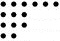
\includegraphics[scale=1]{img/Ferrers_Graph_14.jpg}
\end{center}
Among other things, we may employ Ferrers Graphs to prove that the number of partitions of an integer into exactly $m$ parts equals the number of partitions of the integer into parts, the largest of which is $m$. This is obvious from fact that the transposition of a Ferrers Graph is also a Ferrers Graph and a graph with at most $m$ rows transposing becomes a graph with at most $m$ dots in a row. For example consider the number of partitions of 6 into 4 parts which equates to the number of partitions of 6 with 4 as the largest part:
\begin{center}
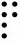
\includegraphics[scale=1]{img/Ferrers_Graph_6(1).jpg} \hspace{.5cm} $\rightarrow$ \hspace{.5cm} 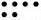
\includegraphics[scale=1]{img/Ferrers_Graph_6(2).jpg}
\end{center}
\begin{center}
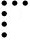
\includegraphics[scale=1]{img/Ferrers_Graph_6(3).jpg} \hspace{.5cm} $\rightarrow$ \hspace{.5cm} 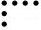
\includegraphics[scale=1]{img/Ferrers_Graph_6(4).jpg}
\end{center}
\end{definition}
\end{minipage}}
\end{center}

\vspace{.3cm}
\section{\textbf{\underline{Recurrence Relations}}}
\vspace{.3cm}
\noindent
Consider the geometric sequence: $\{1,3,3^2,3^3,\dots,3^n,\dots\}$. Clearly, the general term can be expressed as:
\begin{equation*}
a_n = 3^n \hspace{.3cm} \forall n \in \mathbb{Z}^*
\end{equation*}
But we could also express the $n^\text{th}$ term in terms of the other $(n-1)^\text{th}$ term plus a specification of the first term (much like an inductive proof):
\begin{equation*}
a_n = 3a_{n-1} \hspace{.3cm} \text{where} \hspace{.3cm} a_0 = 1
\end{equation*}
The equation $a_n=3a_{n-1}$ is called a recurrence relation for the sequence $\{1,3,3^3,3^3,\dots\}$, and the term $a_0=1$ is called the initial condition. The expression $a_n=3^n$ then represents the solution to the recurrence relation with the stated initial condition. Frequently, counting problems can be expressed by induction as recurrence relations. We first consider methods for translating counting problems into recurrence relations. We then look at techniques for solving recurrence relations. Note that once the recurrence relation is known, by starting with the appropriate initial condition(s) we could iteratively find successive solutions:
\begin{equation*}
\begin{split}
&\text{Given:} \hspace{.3cm} a_n = 3a_{n-1} \hspace{.3cm} \text{where} \hspace{.3cm} a_0 = 1 \\
&\text{Set} \hspace{.1cm} n = 1: \hspace{.3cm} a_1 = 3a_0 = 3 \\
&\text{Set} \hspace{.1cm} n = 2: \hspace{.3cm} a_2 = 3a_1 = 3^2 \\
& \hspace{2.5cm} \vdots
\end{split}
\end{equation*}
This process becomes tedious for large values of $n$, and thus helps to motivate our search for methods of finding a solution. Notice for example that if we know that the solution to the recurrence relation is $a_n = 3^n$ we can solve directly for any choice of $n$ without determining $a_1, a_2, \dots, a_{n-1}$. Although no formal rules can be given, there are definite thought patterns for which are useful to defining recurrence relations.

\begin{example}
Find a recurrence relation for the number of ways, $a_n$, that $n$ distinct objects can be arranged in a row.
\end{example}

\newpage
\begin{solution}
Assume we know $a_{n-1}$ and consider that number of ways of placing the $n^\text{th}$ object. For each one of the $a_{n-1}$ ways of arranging $n-1$ objects, the $n^\text{th}$ object can be inserted before, between, or after giving $n$ new arrangements for each of the $a_{n-1}$ arrangements of $n-1$ objects:
\begin{equation*}
a_n = na_{n-1} \hspace{.3cm} \forall n \in \mathbb{N}
\end{equation*}
We must also deduce an initial condition. We might observe that (by convention) zero objects can be arranged in one way, thus $a_0=1$. Alternatively, we could observe that one object can be arranged in one way, thus $a_1=1$. We could properly state just one of these, though it does not matter which one. Notice that they are both consistent according to the recurrence relation. Let us look at the sequence generated by the recurrence relation and initial condition:
\begin{equation*}
\begin{split}
&\text{Given:} \hspace{.3cm} a_n = na_{n-1} \hspace{.3cm} \text{where} \hspace{.3cm} a_0 = 1 \\
&\text{Set} \hspace{.1cm} n = 1: \hspace{.3cm} a_1 = 1a_0 = 1 \\
&\text{Set} \hspace{.1cm} n = 2: \hspace{.3cm} a_2 = 2a_1 = 2 \\
&\text{Set} \hspace{.1cm} n = 3: \hspace{.3cm} a_3 = 3a_2 = 6 \\
&\text{Set} \hspace{.1cm} n = 4: \hspace{.3cm} a_4 = 4a_3 = 24 \\ 
& \hspace{2.5cm} \vdots
\end{split}
\end{equation*}
These values are of course the same answers that we found when we first encountered this problem. Specifically, $a_n=n!$. Note that this is the solution, and it is easily found inductively.
\end{solution}

\begin{example}
Find a recurrence relation for $a_n$, the number of regions that $n$ straight lines divide the plane into, given that no lines are parallel and no more than 2 meet at any point.
\end{example}
\begin{solution}
First, look at simple cases:
\begin{center}
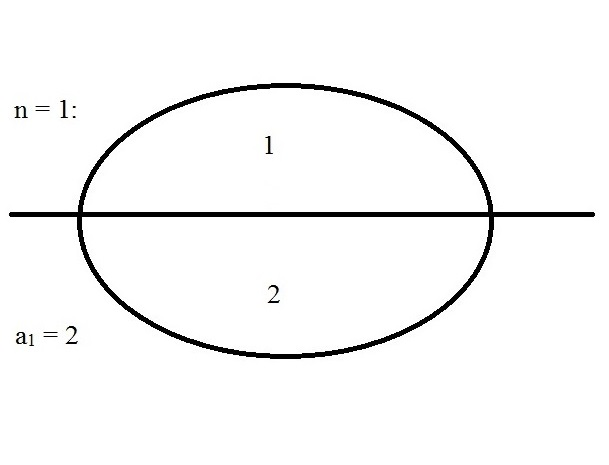
\includegraphics[scale=.3]{img/Example_12_2_1.jpg} 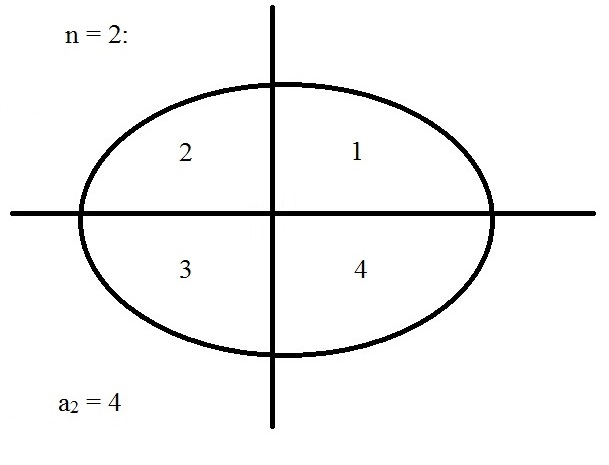
\includegraphics[scale=.3]{img/Example_12_2_2.jpg} 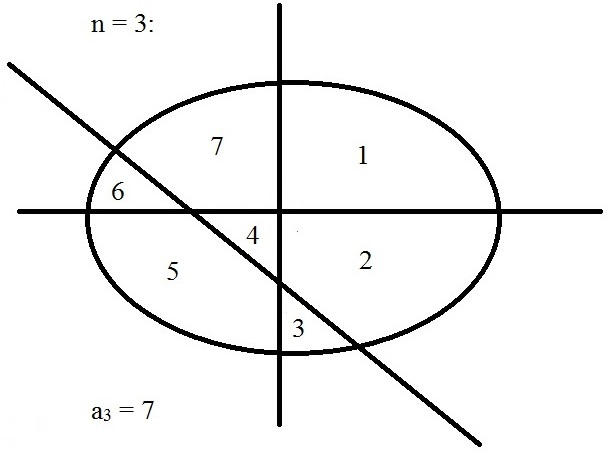
\includegraphics[scale=.3]{img/Example_12_2_3.jpg}
\end{center}
Let us now think inductively. We know that $(n-1)$ lines divide the plane into $a_{n-1}$ regions. When we add that $n^\text{th}$ line, it intersects each of the $(n-1)$ lines once. Thus the $n^\text{th}$ line is divided into $n$ pieces, but each one of these pieces divides an old region into two new regions:
\begin{equation*}
a_n = a_{n-1} + n \hspace{.3cm} \forall n \in \mathbb{N}
\end{equation*}
The initial condition can be taken to be $a_0=1$ because no lines leave the place in 1 piece. Let us check our recurrence relation against the sketches above:
\begin{equation*}
\begin{split}
&\text{Set} \hspace{.1cm} n = 1: \hspace{.3cm} a_1 = a_0 + 1 = 2 \\
&\text{Set} \hspace{.1cm} n = 2: \hspace{.3cm} a_2 = a_1 + 2 = 4 \\
&\text{Set} \hspace{.1cm} n = 3: \hspace{.3cm} a_3 = a_2 + 3 = 7 \\
&\text{Set} \hspace{.1cm} n = 4: \hspace{.3cm} a_4 = a_3 + 4 = 11 \\ 
& \hspace{2.5cm} \vdots
\end{split}
\end{equation*}
\end{solution}

\begin{example}
Find a recurrence relation for $a_n$, the number of different ways that a boy can climb a flight of $n$ steps if he can skip at most one step at a time (that is, he may choose to step up one or two steps at each point).
\end{example}

\newpage
\begin{solution}
First, look at simple cases:
\begin{center}
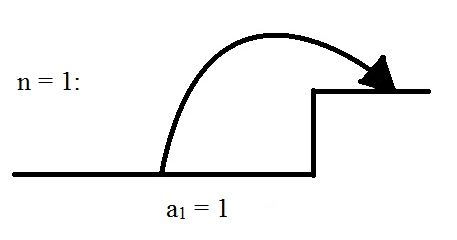
\includegraphics[scale=.3]{img/Example_12_3_1.jpg} 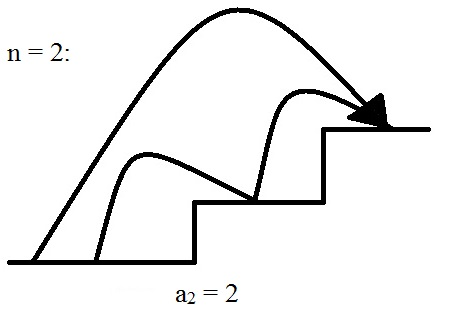
\includegraphics[scale=.3]{img/Example_12_3_2.jpg} 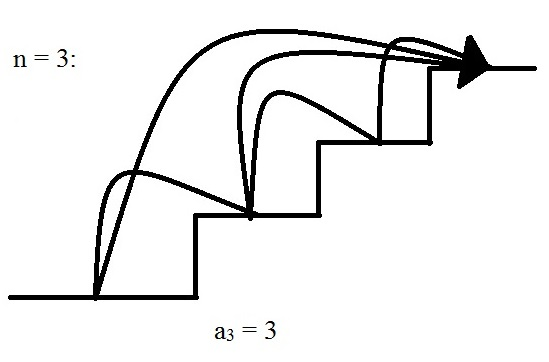
\includegraphics[scale=.3]{img/Example_12_3_3.jpg}
\end{center}
Now try to generalize. Imagine that the boy is confronted by a flight with $n$ steps. He may do one of two mutually exclusive things:
\begin{itemize}

\vspace{.2cm}
\item[(i)]
Step up one step. Then the boy is confronted by a set of $n-1$ steps which can be climbed in $a_{n-1}$ ways.

\vspace{.2cm}
\item[(ii)]
Step up two steps. Then the boy is confronted by a set of $n-2$ steps which can be climbed in $a_{n-2}$ ways

\end{itemize}
Thus the recurrence relation takes the form:
\begin{equation*}
a_n = a_{n-1} + a_{n-2} \hspace{.3cm} \forall n \in \{3, 4, 5, \dots\}
\end{equation*}
The initial conditions follow from the sketches above. Specifically $a_1=1$ and $a_2=2$. This time we need 2 initial conditions. In fact we always need as many initial conditions as the difference between the largest and smallest index in the recurrence relation ($n - (n - 2) = 2$). This quantity is called the order of the recurrence relation. Work out the first few values of $a_n$:
\begin{equation*}
\begin{split}
&\text{Set} \hspace{.1cm} n = 3: \hspace{.3cm} a_3 = a_2 + a_1 = 2 + 1 = 3 \\
&\text{Set} \hspace{.1cm} n = 4: \hspace{.3cm} a_4 = a_3 + a_2 = 3 + 2 = 5 \\ 
&\text{Set} \hspace{.1cm} n = 5: \hspace{.3cm} a_5 = a_4 + a_3 = 5 + 3 = 8 \\ 
& \hspace{2.5cm} \vdots
\end{split}
\end{equation*}
This sequence of numbers occurs so often that it has a name, the Fibonacci sequence: $\{1, 1, 2, 3, 5, 8, 13, 21, 34, \dots\}$. Each number if the sum of the previous two.
\end{solution}

\begin{example}[Two Towers of Hanoi]
Given 3 vertical posts, one of which contains a stack of $n$ decreasing diameter (from bottom to top) discs. Determine the number of moves, $a_n$, required to transfer the stack to another post, observing the following rules:
\begin{itemize}

\vspace{.2cm}
\item[(1)]
Only one disc may be moved at a time

\vspace{.2cm}
\item[(2)]
A larger disc may never be placed on top of a smaller disc

\end{itemize}
\end{example}
\begin{solution}
It takes $a_{n-1}$ moves to move the upper $n-1$ discs onto the second post. It then takes 1 move to move the largest ($n^\text{th}$) disc to the third post. It then takes another $a_{n-1}$ moves to transfer the stack of $(n-1)$ discs so they are on top of the largest disc:
\begin{equation*}
a_n = a_{n-1} + 1 + a_{n-1} = 2a_{n-1} + 1 \hspace{.3cm} \forall n \in \mathbb{N}
\end{equation*}
For the initial condition note that one disc can be moved in one move giving $a_1=1$.
\end{solution}


\begin{example}
Find a recurrence relation for $a_{n,r}$, the number of $r$-permutations which can be formed from $n$ distinct objects.
\end{example}
\begin{solution}
Consider a set of $n-1$ distinct objects:
\begin{itemize}

\vspace{.2cm}
\item[(i)]
$r$ of these can be arranged in $a_{n-1,r}$ ways

\vspace{.2cm}
\item[(ii)]
$r-1$ of these can be arranged in $a_{n-1,r-1}$ ways

\end{itemize}
Now include the $n^\text{th}$ object. If it is not used there are $a_{n-1,r}$ $r$-permutations. If it does get used there are $r a_{n-1,r-1}$ $r$-permutations:
\begin{equation*}
a_{n,r} = a_{n-1,r} + ra_{n-1,r-1} \hspace{.3cm} \text{where} \hspace{.3cm} n > r \hspace{.3cm} \text{and} \hspace{.3cm} r \in \mathbb{N}
\end{equation*}
We will not bother working out the initial conditions for this example.
\end{solution}

\newpage
\begin{example}
Find a recurrence relation for the number of $n$-digit ternary (0,1,2) sequences which contain an even number of zeros.
\end{example}
\begin{solution}
Let $a_n^{(e)} =$ the number of $n$-digit ternary sequences with an even number of zeros and $a_n^{(o)} =$ the number of $n$-digit ternary sequences with an odd number of zeros. Notice further that:
\begin{equation*}
a_n^{(e)} + a_n^{(o)} = 3^n
\end{equation*}
As usual, assume we know $a_{n-1}^{(o)}$ and $a_{n-1}^{(e)}$. Each $(n-1)$-digit sequence contains either an odd or an even number of zeros. If it is even, additional digit added may be a "1" or "2" to keep it even. If it is odd, additional digit added may only be a "0" to make it even. Thus:
\begin{equation*}
\begin{split}
a_n^{(e)} &= 2a_{n-1}^{(e)} + a_{n-1}^{(o)} \\
a_n^{(e)} &= 2a_{n-1}^{(e)} + 3^{n-1} - a_{n-1}^{(e)} \\
a_n^{(e)} &= a_{n-1}^{(e)} + 3^{n-1}
\end{split}
\end{equation*}
The initial condition is given as $a_0^{(e)} = 1$ since no zeros correspond to an even number. The first few values of $a_n^{(e)}$ are:
\begin{equation*}
\begin{split}
&\text{Set} \hspace{.1cm} n = 1: \hspace{.3cm} a_1^{(e)} = 3^0 + a_0^{(e)} = 1 + 1 = 2 \rightarrow [1,2] \\
&\text{Set} \hspace{.1cm} n = 2: \hspace{.3cm} a_2^{(e)} = 3^1 + a_1^{(e)} = 3 + 2 = 5 \rightarrow [00,11,12,21,22] \\ 
& \hspace{2.5cm} \vdots
\end{split}
\end{equation*}
\end{solution}

\vspace{.3cm}
\section{\textbf{\underline{Solving Recurrence Relations}}}
\vspace{.3cm}
\noindent
There is no general procedure for solving recurrence relations so we consider special cases:

\vspace{.3cm}
\begin{center}
\fbox{
\begin{minipage}{7.3 in}
\begin{definition}[Linear, Constant Coefficient, Homogeneous]
Given the following recurrence relation:
\begin{equation*}
a_n = k_1a_{n-1} + k_2a_{n-2} \hspace{.3cm} \forall n \in \{2,3,4,\dots\}
\end{equation*}
and two corresponding initial conditions $a_0$ and $a_1$, the general solution is a linear combination (sum) of terms in the form:
\begin{equation*}
a_n = A\alpha^n
\end{equation*}
where $A$ and $\alpha$ are constants. In order to determine $\alpha$ substitute the above definition into the recurrence relation:
\begin{equation*}
\begin{split}
A\alpha^n &= k_1 A\alpha^{n-1} + k_2 A\alpha_{n-2} \\
0 &= A\alpha^{n-2} \Big[ \alpha^2 - k_1\alpha - k_2 \Big]
\end{split}
\end{equation*}
If $A$ or $\alpha$ are 0, then $a_n = 0$. Since this is not the solution we are looking for we arrive at what is known as the characteristic equation:
\begin{equation*}
\alpha^2 - k_1\alpha - k_2 = 0
\end{equation*}
Using the quadratic formula produces:
\begin{equation*}
\alpha = \frac{1}{2} \Big[ k_1 \pm \sqrt{k_1^2 + 4k_2} \Big]
\end{equation*}
The above states that there are two solutions. If $\alpha_1,\alpha_2 \in \mathbb{R}$ and $\alpha_1 \neq \alpha_2$, then:
\begin{equation*}
a_n = A_1\alpha_1^n + A_2\alpha_2^n
\end{equation*}
Now use the initial conditions to arrive at a system of linear equations which can be solved for the $A$'s:
\begin{equation*}
\begin{split}
a_0 &= A_1\alpha_1^0 + A_2\alpha_2^0 \implies A_1 = (\alpha_2-\alpha_1)^{-1}(\alpha_2 a_0 - a_1) \\
a_1 &= A_1\alpha_1^1 + A_2\alpha_2^1 \implies A_2 = (\alpha_2-\alpha_1)^{-1}(-\alpha_1 a_0 + a_1)
\end{split}
\end{equation*}
\end{definition}
\end{minipage}}
\end{center}

\newpage
\noindent
Note that the $\alpha$'s could also be imaginary. On the other hand if $\alpha_1,\alpha_2 \in \mathbb{R}$ and $\alpha_1=\alpha_2$ the solution is written as: $a_n = A_1\alpha_1^n + A_2 n\alpha_1^n$. To determine the $A$'s, use this solution and the initial conditions. This method works for any order, even though the work above is done for second order. In general if the recurrence relation is of order $r$, then $r$ initial conditions are needed.

\begin{example}
Solve $a_n=3a_{n-1}$ where $n \in \mathbb{N}$ and $a_0=1$.
\end{example}
\begin{solution}
Identify this recurrence relation as being linear, homogeneous, constant coefficient, and of first order. Knowing this, the solution is of the form:
\begin{equation*}
a_n = A\alpha^n
\end{equation*}
Substituting this into the recurrence relation gives:
\begin{equation*}
\begin{split}
A\alpha^n &= 3A\alpha^{n-1} \\
A\alpha^{n-1} \Big[ \alpha - 3 \Big] &= 0
\end{split}
\end{equation*}
In this case the characteristic equation is defined as $\alpha-3=0$ giving $\alpha=3$. Thus the general solution takes the form:
\begin{equation*}
a_n = A(3)^n
\end{equation*}
Use the initial condition to find the value of $A$:
\begin{equation*}
a_0 = 1 = A(3)^0 = A
\end{equation*}
Thus the final solution is:
\begin{equation*}
a_n = 3^n \hspace{.3cm} \forall n \in \mathbb{Z}^*
\end{equation*}
\end{solution}

\begin{example}
Solve $a_n=a_{n-1}+a_{n-2}$ where $n \in \{3,4,5,\dots\}$, $a_1=1$, and $a_2=2$.
\end{example}
\begin{solution}
Assume that the solution is of the form $a_n=A\alpha^n$ and plug into the recurrence relation:
\begin{equation*}
\begin{split}
A\alpha^n &= A\alpha^{n-1} + A\alpha^{n-2} \\
0 &= A\alpha^{n-2} \Big[ \alpha^2 - \alpha - 1 \Big]
\end{split}
\end{equation*}
In this case the characteristic equation is defined as $\alpha^2 - \alpha - 1 = 0$ giving:
\begin{equation*}
\alpha = \frac{1}{2} \Big[ 1 \pm \sqrt{1+4} \Big] = \frac{1}{2} \pm \frac{\sqrt{5}}{2}
\end{equation*}
Thus the general solution takes the form:
\begin{equation*}
a_n = A_1\Big[ \frac{1}{2} + \frac{\sqrt{5}}{2} \Big]^n + A_2\Big[ \frac{1}{2} - \frac{\sqrt{5}}{2} \Big]^n
\end{equation*}
Now before using the initial conditions, to make the calculations easier it can first be found that:
\begin{equation*}
a_0 = a_2 - a_1 = 2 - 1 = 1
\end{equation*}
With this new information the initial conditions are defined as $a_0=1$ and $a_1=1$ giving:
\begin{equation*}
\begin{split}
a_0 = 1 &= A_1\Big[ \frac{1}{2} + \frac{\sqrt{5}}{2} \Big]^0 + A_2\Big[ \frac{1}{2} - \frac{\sqrt{5}}{2} \Big]^0 = A_1 + A_2 \\
a_1 = 1 &= A_1\Big[ \frac{1}{2} + \frac{\sqrt{5}}{2} \Big]^1 + A_2\Big[ \frac{1}{2} - \frac{\sqrt{5}}{2} \Big]^1
\end{split}
\end{equation*}
Solving the system of equations above gives:
\begin{equation*}
a_n = \Big( \frac{1}{2} + \frac{\sqrt{5}}{10} \Big) \Big[ \frac{1}{2} + \frac{\sqrt{5}}{2} \Big]^n + \Big( \frac{1}{2} - \frac{\sqrt{5}}{10} \Big) \Big[ \frac{1}{2} - \frac{\sqrt{5}}{2} \Big]^n
\end{equation*}
Although $a_n$ is written in terms of irrational quantities, $a_n$ itself is an integer as is easily verified.
\end{solution}

\begin{example}
Solve $a_n=4a_{n-1}-4a_{n-2}$ where $n \in \{2,3,4,\dots\}$, $a_0=1$, and $a_1=4$.
\end{example}
\begin{solution}
Assume that the solution is of the form $a_n=A\alpha^n$ and plug into the recurrence relation:
\begin{equation*}
\begin{split}
A\alpha^n &= 4A\alpha^{n-1} - 4A\alpha^{n-2} \\
0 &= A\alpha^{n-2} \Big[ \alpha^2 - 4\alpha + 4 \Big]
\end{split}
\end{equation*}
In this case the characteristic equation is defined as $\alpha^2 - 4\alpha + 4 = 0$ giving:
\begin{equation*}
\alpha = \frac{1}{2} \Big[ 4 \pm \sqrt{16-16} \Big] = 2
\end{equation*}
Thus the general solution takes the form:
\begin{equation*}
a_n = A_1 2^n + A_2 n2^n
\end{equation*}
Use the initial conditions to find the $A$'s:
\begin{equation*}
\begin{split}
a_0 = 1 &= (A_1 + 0A_2)2^0 = A_1 \\
a_1 = 4 &= (A_1 + A_2)2^1 \implies A_2 = 1
\end{split}
\end{equation*}
Thus the final solution is:
\begin{equation*}
a_n = (n+1)2^n
\end{equation*}
\end{solution}

\vspace{.3cm}
\begin{center}
\fbox{
\begin{minipage}{7.3 in}
\begin{definition}[Linear, Unit Coefficient, Non-Homogeneous, $1^\text{st}$ Order]
Given the following recurrence relation:
\begin{equation*}
a_n = a_{n-1} + f_n \hspace{.3cm} \forall n \in \mathbb{N}
\end{equation*}
and an initial condition, $a_0$, to arrive at the solution, first by formal manipulation:
\begin{equation*}
\begin{split}
&\text{Set} \hspace{.1cm} n = 1: \hspace{.3cm} a_1 = a_0 + f_1 = f_0 + f_1 \\
&\text{Set} \hspace{.1cm} n = 2: \hspace{.3cm} a_2 = a_1 + f_2 = f_0 + f_1 + f_2 \\ 
&\text{Set} \hspace{.1cm} n = 3: \hspace{.3cm} a_3 = a_2 + f_3 = f_0 + f_1 + f_2 + f_3 \\ 
& \hspace{2.5cm} \vdots \\
&\text{Set} \hspace{.1cm} n = n: \hspace{.3cm} a_n = a_{n-1} + f_n = f_0 + f_1 + f_2 + \dots + f_n = \sum_{r=0}^n f_r
\end{split}
\end{equation*}
Thus if we set $a_0=f_0$ (the initial condition), then $a_n$ is the $n^\text{th}$ partial sum of the $f_r$. Next define:
\begin{equation*}
\begin{split}
f(x) &= \sum_{r=0}^\infty f_r x^r \\
g(x) &= \sum_{s=0}^\infty x^s = \frac{1}{1-x}
\end{split}
\end{equation*}
where $f(x)$ represents the generating function for $f_r$. It then follows that:
\begin{equation*}
f(x)g(x) = \Bigg[ \sum_{s=0}^\infty x^s \Bigg] \Bigg[ \sum_{r=0}^\infty f_r x^r \Bigg] = \sum_{n=0}^\infty \Bigg[ \sum_{r=0}^n f_r \Bigg] x^n = \sum_{n=0}^\infty a_n x^n
\end{equation*}
In other words, $f(x)g(x)$ is the generating function for the solution to the recurrence relation, $a_n$. This observation provides an expedient method for solving recurrence relations of the form $a_n=a_{n-1}+f_n$ using generating functions.
\end{definition}
\end{minipage}}
\end{center}

\newpage
\begin{example}
Solve $a_n=a_{n-1}+n$ where $n \in \mathbb{N}$ and $a_0=1$.
\end{example}
\begin{solution}
First to identify:
\begin{equation*}
f_n = n \hspace{.3cm} \forall n \in \mathbb{N} \hspace{.3cm} \text{and} \hspace{.3cm} f_0 = a_0 = 1
\end{equation*}
Now to find $f(x)$ in closed form:
\begin{equation*}
\begin{split}
f(x) &= 1 + \sum_{r=1}^\infty rx^r = 1 + x\sum_{r=1}^\infty rx^{r-1} \\
&= 1 + x \frac{d}{dx} \sum_{r=0}^\infty x^r = 1 + x \frac{d}{dx} (1-x)^{-1} \\
&= 1 + \frac{x}{(1-x)^2} = 1 + x(1-x)^{-2}
\end{split}
\end{equation*}
Multiplying by $g(x) = (1-x)^{-1}$ gives:
\begin{equation*}
\begin{split}
f(x)g(x) &= \Big[ 1 + x(1-x)^{-2} \Big] (1-x)^{-1} = (1-x)^{-1} + x(1-x)^{-3} \\
&= \sum_{r=0}^\infty x^r + x\sum_{s=0}^\infty {s+2 \choose 2} x^s = \sum_{r=0}^\infty x^r + \sum_{s=0}^\infty {s+2 \choose 2} x^{s+1} \\
&= 1 + \sum_{n=1}^\infty \Big[ 1 + {n+1 \choose 2} \Big] x^n
\end{split}
\end{equation*}
From the right side it is clear that $a_n = 1 + {n+1 \choose 2}$ where $n \in \mathbb{Z}^*$.
\end{solution}

\begin{example}
Solve $a_n=a_{n-1}+{n \choose 2}$ where $n \in \{2,3,4,\dots\}$ and $a_1=0$.
\end{example}
\begin{solution}
First to identify:
\begin{equation*}
f_n = {n \choose 2} \hspace{.3cm} \forall n \in \{2,3,4\dots,\} \hspace{.3cm} \text{and} \hspace{.3cm} f_0 = f_1 = a_0 = a_1 = 0
\end{equation*}
Now to find $f(x)$ in closed form:
\begin{equation*}
\begin{split}
f(x) &= \sum_{r=2}^\infty {r \choose 2}x^r = \sum_{s=0}^\infty {s+2 \choose 2} x^{s+2} \\
&= x^2 \sum_{s=0}^\infty {s+2 \choose 2} x^s = x^2 \sum_{s=0}^\infty {s+2 \choose s} x^s \\
&= x^2 (1-x)^{-3}
\end{split}
\end{equation*}
Multiplying by $g(x) = (1-x)^{-1}$ gives:
\begin{equation*}
\begin{split}
f(x)g(x) &= x^2 (1-x)^{-4} = x^2 \sum_{j=0}^\infty {j+3 \choose 3} x^j \\
&= \sum_{j=0}^\infty {j+3 \choose 3} x^{j+2} = \sum_{n=2}^\infty {n+1 \choose 3} x^n
\end{split}
\end{equation*}
From the right side it is clear that $a_n = {n+1 \choose 3}$ where $n \in \mathbb{Z}^*$.
\end{solution}

\newpage
\begin{center}
\fbox{
\begin{minipage}{7.3 in}
\begin{definition}[Linear, Constant Coefficient, Non-Homogeneous, $1^\text{st}$ Order]
Given the following recurrence relation:
\begin{equation*}
a_n = ca_{n-1} + f_n \hspace{.3cm} \forall n \in \mathbb{N}
\end{equation*}
and an initial condition, $a_0$, it is easily shown that the solution to this equation consists of a sum of two separate solutions:
\begin{itemize}

\vspace{.2cm}
\item[(1)]
The solution to the associated homogeneous equation:
\begin{equation*}
a_n^* = ca_{n-1}^*
\end{equation*}
as we learned earlier is of the form:
\begin{equation*}
a_n^* = A\alpha^n
\end{equation*}

\vspace{.2cm}
\item[(2)]
A particular solution which depends upon $f_n$, $p_n$. Typical cases include:
\begin{center}
\def\arraystretch{1.5}
\begin{tabular}{| c | c |}
\hline
$f_n$ & $p_n$ \\ \hline
$d$ (constant) & $B$ (constant) \\ \hline
$dn$ & $B_1 n + B_0$ \\ \hline
$dn^2$ & $B_2 n^2 + B_1 n + B_0$ \\ \hline
$d^n$ & $Bd^n$ \\ \hline
\end{tabular}
\end{center}

\end{itemize}
Note that the general solution is then:
\begin{equation*}
a_n = A\alpha^n + p_n
\end{equation*}
and the constant $A$ is evaluated using the initial condition, \underline{after} $p_n$ is determined.
\end{definition}
\end{minipage}}
\end{center}

\begin{example}
Solve $a_n=2a_{n-1}+1$ where $n \in \{2,3,4,\dots\}$ and $a_1=1$.
\end{example}
\begin{solution}
Due to the presence of the coefficient of "2" on $a_{n-1}$, the homogeneous equation must be solved first.
\begin{itemize}

\vspace{.2cm}
\item[(1)]
Homogeneous solution:
\begin{equation*}
a_n^* = 2a_{n-1}^* \implies a_n^* = A2^n
\end{equation*}

\vspace{.2cm}
\item[(2)]
Particular solution: From the table use $p_n = B$:
\begin{equation*}
a_n = 2a_{n-1} + 1 \implies B = 2B + 1 \implies B = -1
\end{equation*}

\vspace{.2cm}
\item[(3)]
General solution = Particular solution + Homogeneous solution:
\begin{equation*}
a_n = a_n^* + B = A2^n - 1
\end{equation*}

\vspace{.2cm}
\item[(4)]
Use the initial condition:
\begin{equation*}
a_1 = 1 = A(2) - 1 \implies A = 1
\end{equation*}
Thus:
\begin{equation*}
a_n = a_n^* + B = 2^n - 1
\end{equation*}

\end{itemize}
\end{solution}

\newpage
\begin{example}
Solve $a_n=3a_{n-1}+2n+1$ where $n \in \{2,3,4,\dots\}$ and $a_1=3$.
\end{example}
\begin{solution}
\hfill
\begin{itemize}

\vspace{.2cm}
\item[(1)]
Homogeneous solution:
\begin{equation*}
a_n^* = 3a_{n-1}^* \implies a_n^* = A3^n
\end{equation*}

\vspace{.2cm}
\item[(2)]
Particular solution: From the table use $p_n = B_1n + B_0$:
\begin{equation*}
a_n = 3a_{n-1} + 2n + 1 \implies B_1n + B_0 = 3(B_1(n-1) + B_0) + 2n + 1 = 3B_1n - 3B_1 + 3B_0 + 2n + 1
\end{equation*}
Sort by power on $n$:
\begin{equation*}
\begin{split}
B_1n &= 3B_1n + 2n \implies B_1 = -1 \\
B_0 &= -3B_1 + 3B_0 + 1 \implies B_0 = -2
\end{split}
\end{equation*}

\vspace{.2cm}
\item[(3)]
General solution = Particular solution + Homogeneous solution:
\begin{equation*}
a_n = a_n^* + B_1n + B_0 = A3^n - n - 2
\end{equation*}

\vspace{.2cm}
\item[(4)]
Use the initial condition:
\begin{equation*}
a_1 = 3 = A(3) - 1 - 2 \implies A = 2
\end{equation*}
Thus:
\begin{equation*}
a_n = a_n^* + B_1n + B_0 = 2(3^n) - n - 2 = 2(3^n - 1) - n
\end{equation*}

\end{itemize}
\end{solution}

\vspace{.3cm}
\section{\textbf{\underline{Graph Theory - Introduction}}}
\vspace{.3cm}
\begin{center}
\fbox{
\begin{minipage}{7.3 in}
\begin{definition}[Graph]
A graph is a figure consisting of points called vertices and straight or curved line segments connecting some or all of the vertices.
\end{definition}
\end{minipage}}
\end{center}

\noindent
A classic example is setup of a sporting competition where vertices represent teams, edges represent matches, and you could even indicate that team A beat team B by indicating a direction on the edge. Ordinarily we indicate vertices by small circles and edges by straight or curved lines. Thus the following two graphs are not the same:
\begin{center}
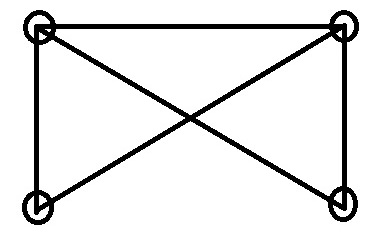
\includegraphics[scale=.3]{img/Graph1_1.jpg} 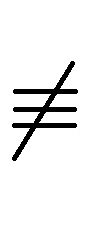
\includegraphics[scale=.3]{img/Not_Equal.jpg} 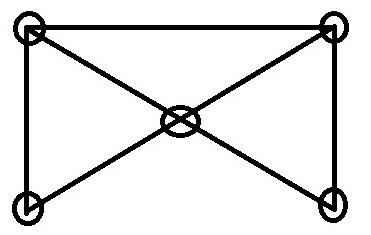
\includegraphics[scale=.3]{img/Graph1_2.jpg}
\end{center}
Though the following are the same (isomorphic):
\begin{center}
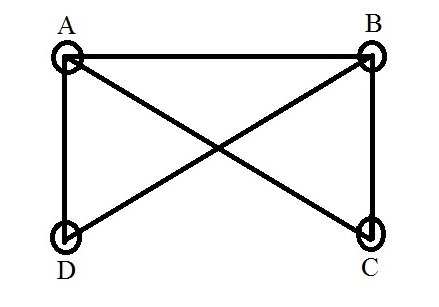
\includegraphics[scale=.3]{img/Graph2_1.jpg} 
\includegraphics[scale=.3]{img/Equal.jpg} 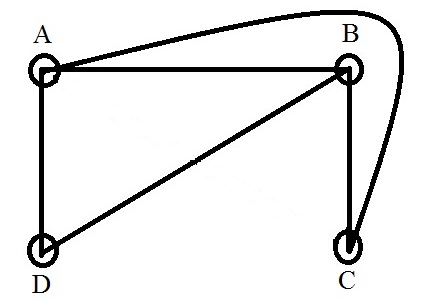
\includegraphics[scale=.3]{img/Graph2_2.jpg} 
\includegraphics[scale=.3]{img/Equal.jpg} 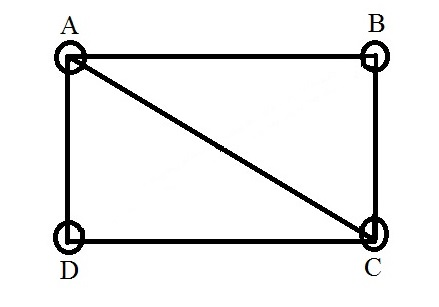
\includegraphics[scale=.3]{img/Graph2_3.jpg}
\end{center}
The important property of any graph is how the vertices are joined by edges, not how it is drawn. Now to mention some special graphs:

\begin{center}
\fbox{
\begin{minipage}{7.3 in}
\begin{definition}[Null Graph]
A graph which consists of $n$ isolated vertices with no edges is called a null graph, $\phi_n$.
\end{definition}
\end{minipage}}
\end{center}

\begin{center}
\fbox{
\begin{minipage}{7.3 in}
\begin{definition}[Complete Graph]
A graph with an edge between every pair of vertices is called a universal or complete graph. If there are $n$ vertices, there will be ${n \choose 2}$ edges, and the graph is called $K_n$.
\end{definition}
\end{minipage}}
\end{center}

\noindent
Every graph, $G_n$, has a complement, $\overline{G}_n$, consisting of the same set of vertices and all edges lacking in $G_n$. Thus $G_n + \overline{G}_n = K_n$, $\overline{(G_n)} \equiv \overline{G}_n$, and $\overline{(\overline{G}_n)} = G_n$.

\newpage
\section{\textbf{\underline{Connected Graphs}}}
\vspace{.3cm}
\noindent
Imagine that we have before us a graph $G$, which need not be planar. Assume that we start at a vertex $A$ and proceed along an edge to vertex $B$, then along another to vertex $C$, etc. No restrictions are placed on our travel as we may pass through any vertex several times, travel along any edge more than once and in either direction. If in our travels we arrive at vertex $T$, then $T$ is \underline{connected} to $A$. If we have passed through any vertex more than once, we can shorten our route from $A$ to $T$ by eliminating the circular part of the route. A route from $A$ to $T$ with the circular parts removed, so each vertex between $A$ and $T$ is visited only once is called an \underline{arc}. A route which has no edges transversed more than once, though vertices may have been visited more than once (along different edges) is called a \underline{path}. A path which returns to its starting point is called a \underline{cyclic} or \underline{circular path}. An arc which returns to its starting point is called a \underline{circuit}.






\end{document}